\documentclass{beamer}

\usetheme{Madrid}

\usepackage{lipsum}
\usepackage{multicol}
\usepackage{listings}
\usepackage{multirow}

% Define a custom color
\definecolor{backcolour}{rgb}{255,255,255}
\definecolor{codegreen}{rgb}{0,0.6,0}

% Define a custom style
\lstdefinestyle{myStyle}{
    backgroundcolor = \color{backcolour},   
    commentstyle = \color{codegreen},
    basicstyle=\linespread{0.4}\tiny,
    breakatwhitespace=false,         
    breaklines=true,        
    keepspaces=true,                               
    showspaces=false,                
    showstringspaces=false,
    showtabs=false,                  
    tabsize=2,
}

% Use \lstset to make myStyle the global default
\lstset{style=myStyle}

\usepackage{graphicx}
\usepackage{listings}
\usepackage{verbatim}
\linespread{1.5}
\usepackage{pgfplots}
\usepackage{tikz}

\usepackage{amsmath, amsthm, amssymb, latexsym}

%\newtheorem{definition}{Definition}

\newcommand{\pathtoimages}{/Users/charlesrambo/Desktop/Bootcamp24/Images}

\title{Unit 3: Combinatorics, Probability, and Statistics}
\author{Charles Rambo}
\institute{UCLA Anderson}
\date{2024}


\begin{document}
\input{systempreamble}


\frame{\titlepage}

\begin{frame}[allowframebreaks]

\frametitle{Table of Contents}
\tableofcontents
\end{frame}


\section{Combinatorics}

\begin{frame}
\begin{center}
\Huge Combinatorics
\end{center}
\end{frame}


\begin{frame}

\frametitle{Combinatorics}
\begin{Definition}
{\bf Combinatorics} is the branch of mathematics concerned with counting.
\end{Definition}
The fundamental counting principle states:
\begin{quote}
If there are $m_k$ ways to make the $k$-th decision for $k = 1, 2,\ldots n$, then there are a total of 
$$
\prod_{k = 1}^n m_k = m_1\cdot m_2\cdot\ldots\cdot m_n
$$ 
ways to make the $n$ independent decisions. 
\end{quote}
\end{frame}

\begin{frame}[t]
\frametitle{Combinatorics Example}
\small
\begin{Example}
Let's say that the personal code for your bank pin consists of six characters, each of which can be any letter or numerical digit.
\begin{enumerate}
\item[(a)] How many possible personal codes are there?
\item[(b)] Suppose you want your pin to have no repeated characters. How many possible pins would there be now?
\end{enumerate}
\end{Example}
\end{frame}

\subsection{Permutations and Combinations}

\begin{frame}
\frametitle{Permutations and Combinations}
\begin{Definition}
If the order in which the objects are chosen matters, each complete selection of $k$ objects from an original $n$ is called a {\bf permutation}. If the order does not matters, then each complete selection is called a {\bf combination}.
\end{Definition} 

\end{frame}

\begin{frame}
\frametitle{Permutations and Combinations without Repetition}

The number of {\it permutations} of $k$ elements from a selection of $n$ {\it without repetition} is 
$$
_n P_k = \frac{n!}{(n - k)!}.
$$
The number of {\it combinations} of $k$ elements from a selection of $n$ {\it without repetition} is 
$$
_nC_k = {n\choose k} =  \frac{n!}{k!(n-k)!}.
$$

\end{frame}

\begin{frame}[t]
\frametitle{Permutations and Combinations without Repetition}
\begin{Example}
\begin{enumerate}
\item[(a)] Among eight comparable investment funds, {\it ex ante}, how many different ways are there to list the top three performing funds?
\item[(b)] How may three-element subsets does a set of nine elements have?
\end{enumerate}
\end{Example}
\end{frame}

\begin{frame}
\frametitle{$n$ Elements of $k$ Types}
Suppose there are $n_k$ indistinguishable elements of type $k$, where $k = 1, 2,\ldots m$. Let
$$
n = n_1 + n_2 + \ldots + n_m.
$$
Then the number of {\it unique} rearrangements of the $n$ elements is
$$
{n \choose n_1, n_2,\ldots, n_m} = \frac{n!}{n_1! n_2!\ldots n_m!}.
$$
\end{frame}

\begin{frame}[t]
\frametitle{$n$ Elements of $k$ Types}
\begin{Example}
How many unique rearrangements of the letters in the word BANANA are there?
\end{Example}
\end{frame}


\subsection{Stars-and-Bars}

\begin{frame}
\frametitle{Stars-and-Bars}

\begin{Theorem}[Stars-and-Bars]
Suppose there are $k$ types of items. If the order in which items are selected does not matter, the number of ways to select $n$ items is
$$
{n + k - 1\choose k - 1} = {n + k - 1\choose n}.
$$
\end{Theorem}
\end{frame}

\begin{frame}[t]
\frametitle{Stars-and-Bars Example}
\begin{Example}
In how many ways can we write the number 11 as the sum of five positive integers?
\end{Example}
\end{frame}

\begin{frame}
\frametitle{Stars-and-Bars on YouTube}
\small 
Watch Ken Ribet explain Stars-and-Bars (\url{https://youtu.be/UTCScjoPymA}).
\begin{center}
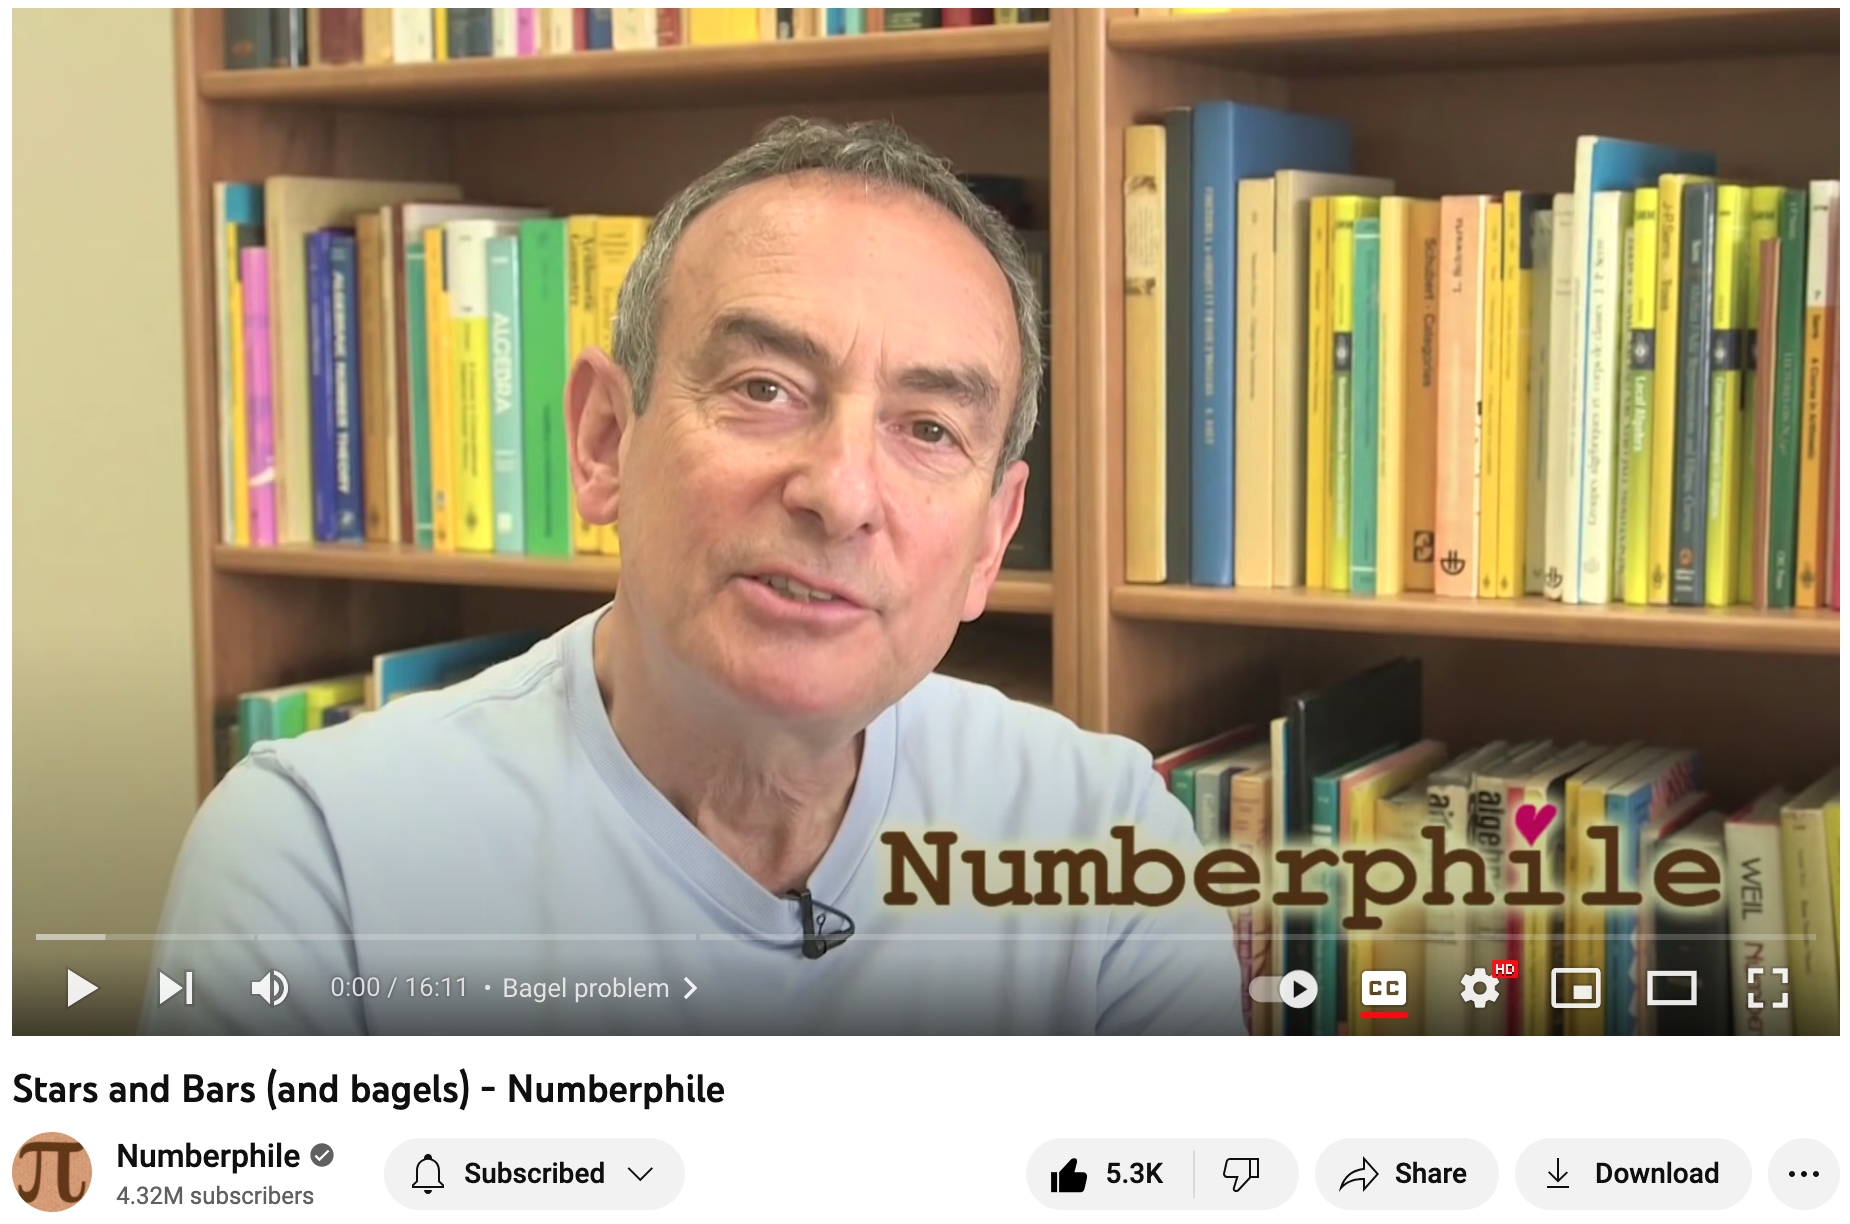
\includegraphics[scale = 0.25]{\pathtoimages/ribet.png}
\end{center}

\end{frame}

\subsection{The Pigeonhole Principle}

\begin{frame}
\frametitle{The Pigeonhole Principle}

\begin{Theorem}[Pigeonhole Principle]
Suppose there are $n$ objects distributed among $m$ sets, where $n \geq m$. Then one set must contain at lest $\lceil n/m \rceil$ elements.
\end{Theorem}
\end{frame}

\begin{frame}[t]
\frametitle{The Pigeonhole Principle Example}
\begin{Example}
Suppose we have a set of $n + 1$ whole numbers. Show that we can always select two elements $a$ and $b$ such that $a - b$ is divisible by $n$.
\end{Example}

\end{frame}

\subsection{Inclusion--Exclusion Principle}

\begin{frame}
\frametitle{Inclusion--Exclusion Principle}

\begin{Theorem}[Inclusion--Exclusion Principle]
Suppose $|A|$ denotes the number of elements in $A$. Consider finite sets $A_1$ and $A_2$. The number of elements in $A_1\cup A_2$ is
$$
|A_1\cup A_2| = |A_1| + |A_2| - |A_1\cap A_2|.
$$
More generally, for $A_1, A_2,\ldots A_n$, the number of elements in $\displaystyle\bigcup_{i = 1}^n A_i$ is
\begin{align*}
\left|\bigcup_{i = 1}^n A_i\right| &= \sum_{i = 1}^n |A_i| - \sum_{1 \leq i < j \leq n} \left|A_i\cap A_j \right|+ \sum_{1\leq i < j < k\leq n} \left| A_i \cap A_j \cap A_k\right|\\
						&\qquad  - \ldots + (-1)^{n +1} \left|A_1\cap A_2\cap \ldots \cap A_n\right|.
\end{align*}
\end{Theorem}
\end{frame}

\begin{frame}[t]
\frametitle{Inclusion--Exclusion Principle Example}
\tiny
\begin{Example}
There are 100 students enrolled in the UCLA MFE class of 2025. Sixty-five students are taking statistical arbitrage, 43 are taking credit markets, and 37 are taking behavioral finance. If 23 students are taking statistical arbitrage and credit markets, 15 are taking statistical arbitrage and behavioral finance, and 20 are taking credit markets and behavioral finance, how many students are taking all three classes?
\end{Example}
\end{frame}

\section{Probability}

\begin{frame}
\begin{center}
\Huge Probability
\end{center}
\end{frame}

\begin{frame}
\frametitle{$\boldsymbol\sigma$-Algebra}
\begin{Definition}
Let $\Omega$ be some set, and let $2^\Omega$ represent the set of all subsets of $\Omega$. Then a subset $\mathcal{F}$ of $2^\Omega$ is called a $\boldsymbol\sigma$-{\bf algebra} if and only if it satisfies the following three properties:
\medskip

\begin{quote}
\begin{enumerate}
\item[SA.1] $\Omega$ is in $\mathcal{F}$.
\item[SA.2] If $A\in \mathcal{F}$ then $A^c = \{x\in\Omega: x\not\in A\}  \in\mathcal{F}$.
\item[SA.3] If $A_k\in\mathcal{F}$ for $k = 1, 2,\ldots$, then $\displaystyle\bigcup_{k= 1}^\infty A_k\in\mathcal{F}$.
\end{enumerate}
\end{quote}
\end{Definition}
\end{frame}

\begin{frame}
\frametitle{Probability Definition}
\begin{Definition}
Let $\Omega$ be a set and let $\mathcal{F}$  be a $\sigma$-algebra of $\Omega$. A {\bf probability} is defined as a function $P:\mathcal{F}\to [0, 1]$ if the following hold:
\medskip

\begin{quote}
\begin{enumerate}
\item[P.1] $P(\varnothing) = 0$.
\item[P.2] $P(\Omega) = 1$.
\item[P.2] For $E_k \in\mathcal{F}$ and $E_k\cap E_\ell= \varnothing$ for $k\neq \ell$, we have
$$
P\left(\bigcup_{k = 1}^\infty E_k\right) = \sum_{k = 1}^\infty P(E_k).
$$
\end{enumerate}
\end{quote}
We typically call $\Omega$ the {\bf sample space}. The elements of $\mathcal{F}$ are called {\bf events}. Altogether, $(\Omega, \mathcal{F}, P)$ forms a {\bf probability space}.
\end{Definition}
\end{frame}

\begin{frame}[t]
\frametitle{Probability Example}
\begin{Example}
Consider the sample space $[0, 1]\times [0, 1]$. We define $P:\mathcal{F}\to [0, 1]$ such that $P(E) = \text{area}(E)$. In this cases, we would have 
$$
\mathcal{F} = \{E \subseteq [0, 1]\times [0, 1]: \text{area of}\ E\ \text{exists}\}.
$$
We need $\mathcal{F}$ because there are subsets of $[0, 1]\times [0, 1]$ whose area can't be measured!
\end{Example}
\end{frame}

\begin{frame}
\frametitle{Properties of Probability Measure}
Consider the probability space $(\Omega, \mathcal{F}, P)$. Suppose $A$ and $B$ are in $\mathcal{F}$.
\begin{itemize}
\item $A \subseteq B$ implies $P(A) \leq P(B)$
\item $P(A^c) = 1 - P(A)$
\item $P(A\cup B) = P(A) + P(B) - P(A\cap B)$
\end{itemize}
\end{frame}

\begin{frame}[t]
\frametitle{Probability Example}
\small
\begin{Example}
The point $(x, y)$ is selected at random from $[0, 1]\times [0, 1]$. Assume that all points within the sample space are equally likely to be selected. What is the probability that $xy$ is less than 1/2?
\end{Example}


\end{frame}

\subsection{Conditional Probabilities}

\begin{frame}
\frametitle{Conditional Probabilities}
\begin{Definition}
If the occurrence of the event $A$ depends on the occurrence of $B$ then the conditional probability is
$$
P(A | B) = \frac{P(A\cap B)}{P(B)}
$$
whenever $P(B) > 0$. If $P(B) = 0$ the conditional probability is undefined.
\end{Definition}

\end{frame}

\begin{frame}[t]
\frametitle{Conditional Probability Example}
\begin{center}
\tiny
\begin{tabular}{c | c c c}
\hline
{\bf Credit}		&	{\bf Excellent}	&	{\bf Good}	&	{\bf Poor}\\\hline
{\bf Defaults}		&	930			&	1,350	&	5,856\\
{\bf Non-Defaults}	&	10,321		&	18,007	&	13,536
\end{tabular}
\end{center}
\begin{Example}
\tiny
A loan originator has a 50,000 observation loan data set. This originator places applicants' credit into one of three categories: excellent, good, and poor. Details about this data set are shown above. What is the probability of default given that an applicant's credit is placed into the category good?
\end{Example}
\end{frame}

\begin{frame}
\frametitle{Bayes' Rule}

\begin{Theorem}[Bayes]
Suppose $P(B) > 0$. Then
$$
P(A|B) = \frac{P(B|A) P(A)}{P(B)}.
$$
\end{Theorem}

\begin{Theorem}[Law of Total Probabilities]
Suppose $B_i \cap B_j = \varnothing$ for $i\neq j$ and $\displaystyle\bigcup_{i = 1}^n B_i = \Omega$. Then
$$
P(A) = P(A|B_1) P(B_1) + P(A|B_2)P(B_2) + \ldots + P(A|B_n) P(B_n).
$$
\end{Theorem}

\end{frame}

\begin{frame}[t]
\frametitle{Bayes' Rule Example}
\small
\begin{Example}
Assume the probability that an unskilled asset manager beats the market is 50\%, and the probability that a skilled asset manager beats the market is 60\%. If 10\% of asset managers are skilled, what is the probability that an asset manager is skilled given that she beats the market?
\end{Example}

\end{frame}

\begin{frame}
\frametitle{Bayes' Rule on YouTube}
Watch the StatQuest video about Bayes' theorem (a.k.a. Bayes' rule) on YouTube (\url{https://youtu.be/9wCnvr7Xw4E}).
\begin{figure}
\centering
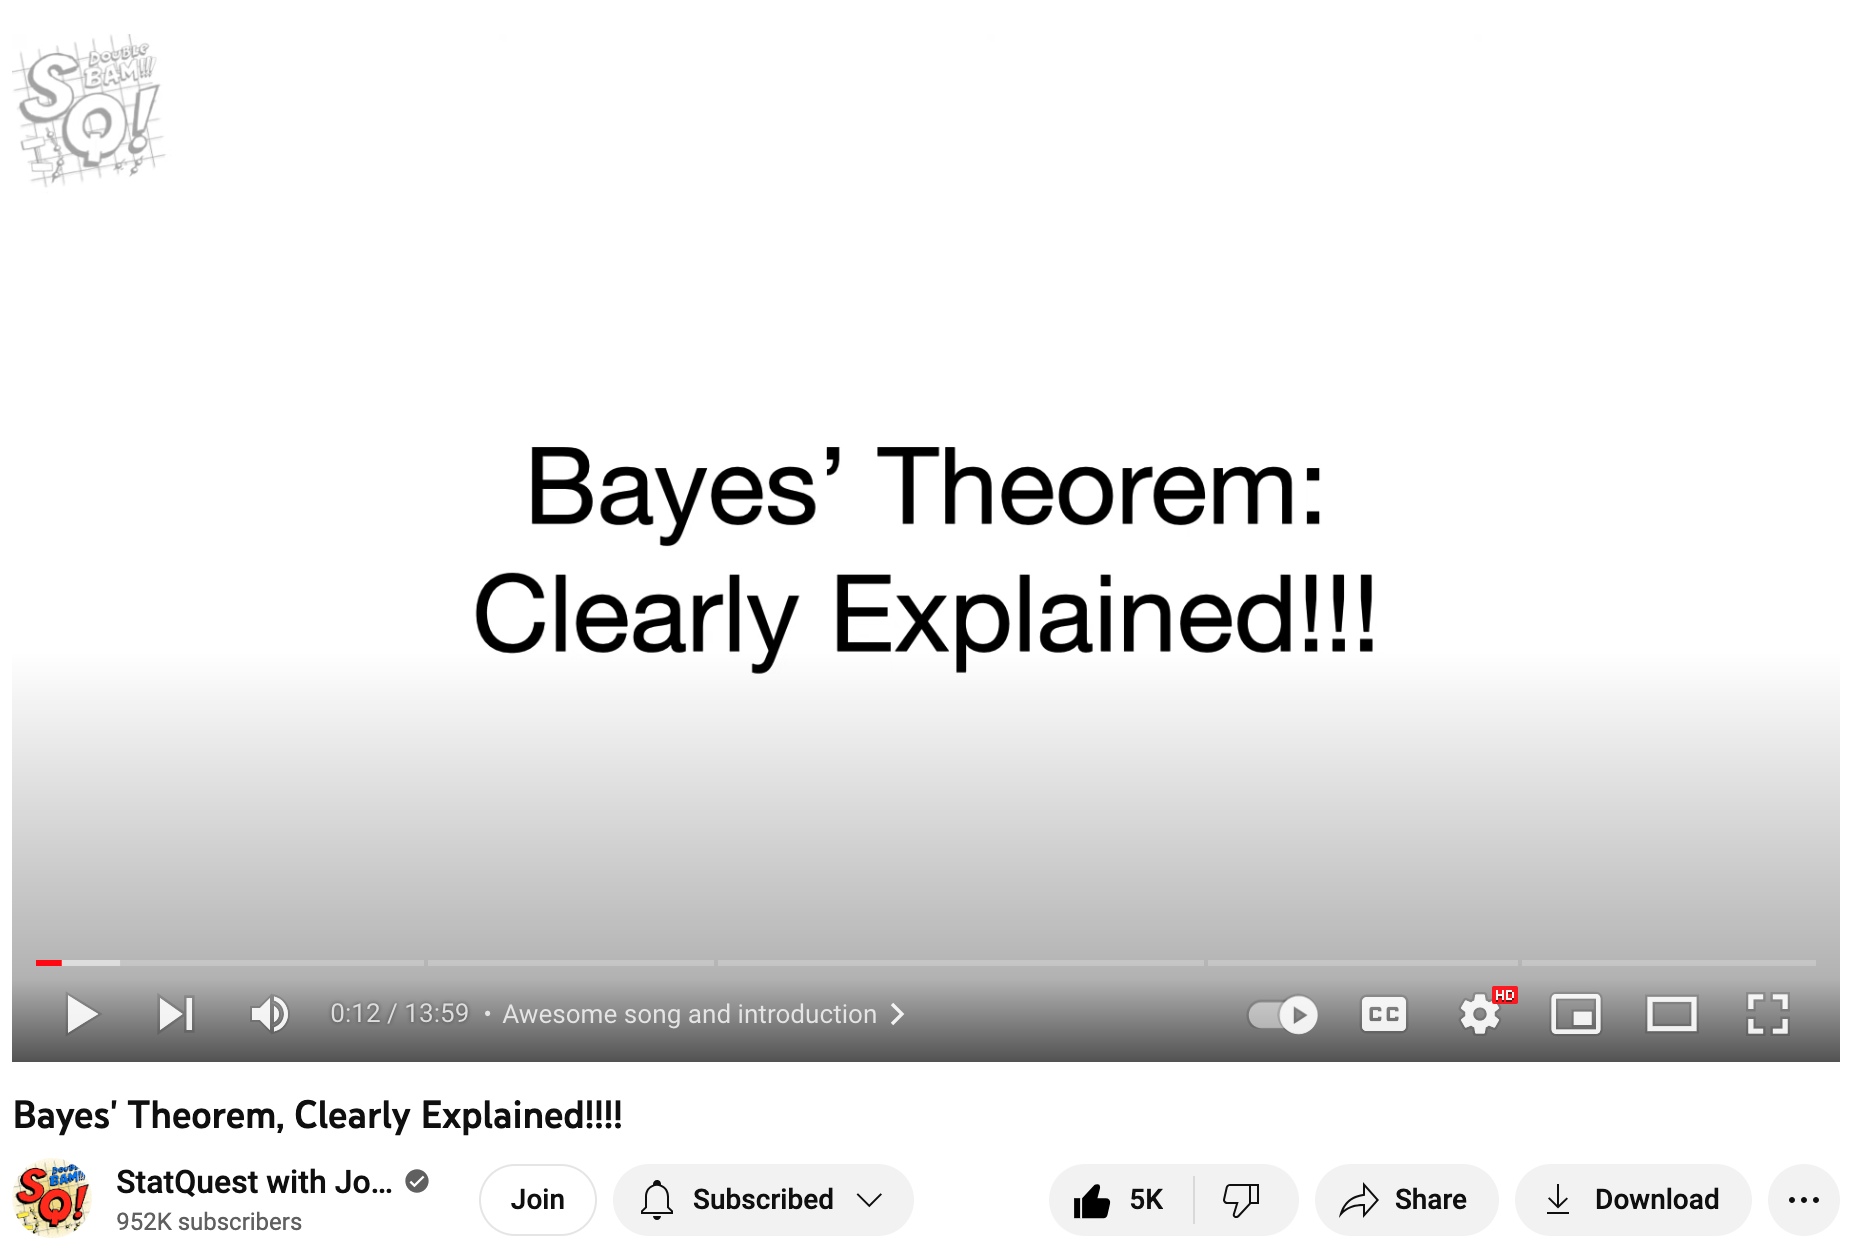
\includegraphics[scale = 0.25]{\pathtoimages/bayes_statquest.png}
\end{figure}

\end{frame}

\begin{frame}
\frametitle{Independent Events}

\begin{Definition}
Events $A$ and $B$ are independent if $P(A|B) = P(A)$.
\end{Definition}
If two events are independent then it's easy to prove
$$
P(A\cap B) = P(A) P(B).
$$
\end{frame}

\begin{frame}[t]
\frametitle{Independent Events Example}
\small
\begin{Example}
One urn contains four red balls and six blue balls. A second urn contains sixteen red balls and $x$ blue balls. A single ball is drawn from each urn. The probability that both balls are the same color is 0.44 . Calculate $x$.
\end{Example}

\end{frame}

\subsection{Random Variables} 

\begin{frame}
\frametitle{Random Variables}

\begin{Definition}
A random variable $X$ is a function $X:\Omega\to\mathbb{R}$ where $P\left(X^{-1}(A)\right)$ exists for each $A\subseteq\mathbb{R}$.
\end{Definition}

The probability that $X$ takes on values in the subset $S$ of $\mathbb{R}$ is written
$$
P(X\in S) = P\left(\{\omega \in\Omega : X(\omega)\in S\}\right).
$$
The probability that $X$ takes on value $x$ in $\mathbb{R}$ is written
$$
P(X = x) = P\left( \{\omega \in\Omega : X(\omega) = x\} \right).
$$
\end{frame}

\begin{frame}
\frametitle{Types of Random Variables}
There are three types of random variables: {\it discrete} random variables, {\it continuous} random variables, and {\it mixed} random variables. 
\begin{itemize}
\item A discrete random variable is a random variable whose range is either finite or countably infinite. 
\item A continuous random variable is a random variable whose range is uncountable.
\item A mixed random variable is partially discrete and partially continuous.
\end{itemize}

\end{frame}

\begin{frame}[t]
\begin{Example}
State whether the random variables are discrete, continuous, or mixed.
\begin{enumerate}
\item[(a)] A coin is tossed ten times. The random variable $X$ is the number of tails.
\item[(b)] The random variable $Y$ measures the time until a firm defaults on its debt.
\item[(c)] The random variable $Z$ measures the time, in years, until a firm defaults on a particular bond that matures in $T$ years. If the firm meets all of its payment obligations for the bond, $Z$ is given a value of $T$.
\end{enumerate}
\end{Example}

\end{frame}

\subsection{Discrete Random Variables}

\begin{frame}
\frametitle{Probability Mass Function}
\begin{Definition}
For a discrete random variable $X$, we define the {\bf probability mass function} or {\bf pmf} by the equation
$$
p(x) = P(X = x).
$$
\end{Definition}
\end{frame}

\begin{frame}[t]
\frametitle{Probability Mass Function Example}
\begin{Example}
A coin is flipped three times. Let the random variable $X$ denote the number of heads. Find the pmf of $X$.
\end{Example}

\end{frame}

\begin{frame}
\frametitle{Cumulative Distribution Function}
\begin{Definition}
For a discrete random variable $X$, we define the {\bf cumulative distribution function} or {\bf cdf} as
$$
F(x) = P(X\leq x) = \sum_{t \leq x} P(X = t).
$$
\end{Definition}
\end{frame}

\begin{frame}[t]
\frametitle{Probability Mass Function Example}
\begin{Example}
The random variable $X$ denotes the number selected from the set $\{1, 2, 3, 4\}$. If each number is equally likely, find the cdf.
\end{Example}

\end{frame}

\begin{frame}
\frametitle{Discrete Uniform Distribution}
\begin{Definition}
The {\bf discrete uniform distribution} is a symmetric probability distribution. In this distribution, a finite number of values are equally likely to be observed. Every one of the $n$ values has equal probability $1/n$ of being observed.
\end{Definition}
\end{frame}

\begin{frame}
\frametitle{Binomial Distribution}
\small 
\begin{Definition}
The {\bf binomial distribution} with parameters $n$ and $p$ is the discrete probability distribution of the number of successes in a sequence of $n$ independent experiments, each ending in either success with probability $p$ or failure with probability $q = 1- p$.
\end{Definition}
To denote that $X$ is a binomial random variable with parameters $n$ and $p$, we write $X\sim{\mathcal{B}(n, p)}$. The probability 
$$
\displaystyle P(X = x) = \begin{cases}{n\choose x} p^x q^{n - x},	&	x = 0, 1, \ldots, n\\ 0,	&\text{otherwise.}\end{cases}
$$
\end{frame}

\begin{frame}[t]
\frametitle{Binomial Distribution Example}
\small
\begin{Example}
Suppose a portfolio manager has a portfolio of 25 high yield bonds. She assumes that each bond has a one-year default probability of 5\%. Her portfolio is well diversified so defaults are independent. What is the probability that more than one bond defaults?
\end{Example}
\end{frame}

\begin{frame}[fragile]
\frametitle{Binomial Distribution Python Example}
\begin{Example}
Use Python to check the previous result by simulating the event 100,000 times. 
\end{Example}

\begin{lstlisting}[language=Python]
import numpy as np
from scipy.stats import binom

# Generate 100,000 simulations
defaults = binom.rvs(n = 25, p = 0.05, loc = 0, size = 100_000, random_state = 0)

# Calculate probability
prob = np.mean(defaults > 1)

print(f'The probability that more than one bond defaults is {prob:.3f}.')
\end{lstlisting}
The output is 0.357.

\end{frame}

\begin{frame}
\frametitle{Poisson Distribution}
\begin{Definition} 
The {\bf Poisson distribution} is a discrete probability distribution that expresses the probability of a given number of events $x$ occurring in a fixed interval if these events occur independently with a constant rate $\lambda$.
\end{Definition}
To denote that $X$ is a Poisson random variable with parameter $\lambda$, we write $X\sim{\mathcal{P}(\lambda)}$. The probability 
$$
P(X = x) = \begin{cases} \dfrac{\lambda^x e^{-\lambda}}{x!},&  x = 0, 1, 2,\ldots\\ 0,	&	\text{otherwise.}\end{cases}
$$
\end{frame}

\begin{frame}[t]
\frametitle{Poisson Distribution Example}
\tiny
\begin{Example}
After graduation from the MFE program, you become a famous and successful portfolio manager. To help younger men and women succeed in finance, you begin writing a memoir of your life. In the first draft of your book, there are an average of three spelling errors per page. Suppose that the number of errors per page follows a Poisson distribution. What is the probability of having no errors on a page?
\end{Example}

\end{frame}

\subsection{Continuous Random Variables}

\begin{frame}
\frametitle{Continuous Random Variables}
\begin{Definition}
We say that a random variable $X$ is {\bf continuous} if there exists a non-negative function $f$ defined for all real numbers and having the property that for any set $B$ of real numbers we have
$$
P(X\in B) = \int_B f(x)\ dx.
$$
The function $f$ is called the {\bf probability density function} or {\bf pdf} of the random variable $X$.
\end{Definition}

\end{frame}

\begin{frame}
\frametitle{Diagram}
\begin{center}
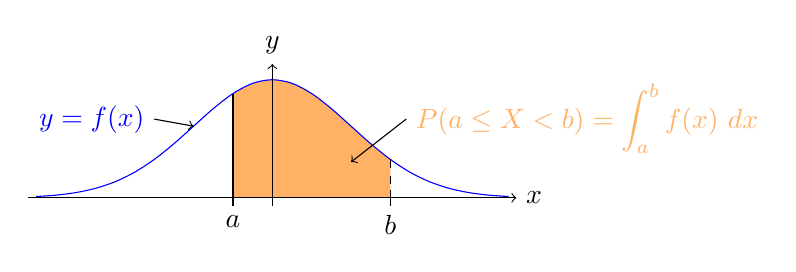
\begin{tikzpicture}[declare function = {normal(\x) = 1.5 * exp(-0.5 * \x * \x);}, ]

% Shade orange area underneath curve.
\fill [fill=orange!60] (-0.5, 0) -- plot[domain= -0.5:1.5] (\x, {normal(\x)}) -- (1.5 ,0) -- cycle;

% Draw and label normal distribution function
\draw[color=blue, domain=-3:3, smooth] plot (\x, {normal(\x)});

% Draw line
\draw (-0.5, {normal(-0.5)}) -- (-0.5, 0);
\draw (-0.5, 0.1) -- (-0.5, -0.1) node[below] {$a$}; 

% Add dashed line dropping down from normal.
\draw[dashed] (1.5, {normal(1.5)})  -- (1.5, 0);
\draw (1.5, 0.1) -- (1.5, -0.1) node[below] {$b$};

\draw[->] (-3.1, 0) -- (3.1, 0) node[right] {$x$};
\draw[->] (0, -0.1) -- (0, 1.7) node[above] {$y$};

\draw [<-] (1, {0.5 * normal(1)}) -- (1.7, 1) node[right] {$\textcolor{orange!60}{ P(a\leq X < b) = \displaystyle\int_a^b f(x)\ dx}$};
\draw[<-] (-1, {normal(-1)}) -- (-1.5, 1) node[left] {$\textcolor{blue}{y = f(x)}$};

\end{tikzpicture}
\end{center}
\end{frame}

\begin{frame}
\frametitle{Cumulative Distribution Function}
\begin{Definition}
The {\bf cumulative distribution function} or {\bf cdf} of a random variable $X$ is defined to be
$$
F(x) = P(X \leq x) = \int_{-\infty}^x f(t)\ dt,
$$
where $f$ is the pdf of $X$.
\end{Definition} 

\end{frame}

\begin{frame}
\frametitle{Properties of CDFs}
\small
The cumulative distribution function $F$ of a continuous random variable $X$ with probability density function $f$ satisfies the following properties.
\begin{multicols}{2}
\begin{enumerate}
\item[(a)] $0 \leq F(x) \leq 1$
\item[(b)] If $x_1 < x_2$, then $F(x_1) < F(x_2)$
\item[(c)] $\displaystyle\lim_{x\to-\infty} F(x) = 0$
\item[(d)] $\displaystyle\lim_{x\to\infty} F(x) = 1$
\item[(e)] $P(a < X \leq b) = F(b) - F(a)$
\item[(f)] $F$ is continuous 
\item[(g)] $F'(x) = f(x)$ whenever $F'$ exists
\end{enumerate}
\end{multicols}
All of these, except (g), hold for discrete random variables as well.
\end{frame}

\begin{frame}[t]
\frametitle{PDF and CDF Example}
\begin{Example}
Suppose a random variable $X$'s pdf is proportional to $x^2$ on the interval $[-1, 2]$ and 0 elsewhere. Find the pdf and cdf of $X$.
\end{Example}

\end{frame}

\begin{frame}
\frametitle{The Continuous Uniform Distribution} 
\small 
\begin{Definition}
The {\bf continuous uniform distributions} describes an experiment where there is an arbitrary outcome that lies between certain bounds. The bounds are defined by the parameters $a$ and $b$, which are the minimum and maximum values. The interval can either be closed or open. The distribution is often abbreviated $\mathcal{U}(a, b)$. 
\end{Definition}
The pdf and cdf of the continuous uniform distribution on $[a, b]$ are
$$
f(x) = \begin{cases} \displaystyle\frac{1}{b - a},	&	a\leq x\leq b\\ 0, & \text{otherwise}\end{cases}\qquad\text{and}\qquad F(x) = \begin{cases} 0,	&	x < a\\ \displaystyle\frac{x - a}{b - a}, & 	a\leq x\leq b\\	1,	&	x > b.\end{cases}
$$
\end{frame}

\begin{frame}[t]
\frametitle{Continuous Uniform Distribution Example}
\begin{Example}
Suppose that $X\sim{\mathcal{U}(0, b)}$, where $b > 1$. Find $P(X^2 < X)$.
\end{Example}

\end{frame}

\begin{frame}
\frametitle{Normal Distribution}
\begin{Definition}
The {\bf normal} or {\bf Gau{\ss}ian distribution} has probability density function 
$$
\displaystyle f(x) = \frac{1}{\sigma \sqrt{2\pi}} e^{-\frac{1}{2}\left(\frac{x - \mu}{\sigma}\right)^2}.
$$
The parameters of the distribution are $\mu$ and $\sigma^2$. To denote that $X$ follows a normal distribution, we write $X\sim{\mathcal{N}(\mu, \sigma^2)}$.
\end{Definition} 
\end{frame}

\begin{frame}[fragile]
\frametitle{Normal Python Example}
\small
\begin{Example}
Use Python to illustrate how $\mu$ and $\sigma$ affect the graph of the pdf.
\end{Example}

\begin{lstlisting}[language=Python]
import numpy as np, matplotlib.pyplot as plt
from scipy.stats import norm

# Use LaTeX
plt.rcParams['text.usetex'] = True

# Use Seaborn style
plt.style.use('seaborn')

# Mu- and sigma-values
mu_vals, sigma_vals = [-2, 0, 1], [0.5, 1, 1.5]

# Set up subplots
fig, ax = plt.subplots(1, 2, sharey = True, figsize = (10, 6))

# Get x-values
x_vals = np.linspace(-4.5, 3.5, 100)
\end{lstlisting}

\end{frame}

\begin{frame}[fragile]
\frametitle{Normal Python Example}
\begin{lstlisting}[language=Python]
# Loop over mu-values
for mu in mu_vals:

    # Note norm.pdf vectorized
    y_vals = norm.pdf(x_vals, loc = mu, scale = 1)
    
    ax[0].plot(x_vals, y_vals, label = r'$\mu =$ ' + str(mu))

# Create legend for first subplot
ax[0].legend()

# Loop over sigma-values
for sigma in sigma_vals:
    
    # Note norm.pdf vectorized; also scale is std not var
    y_vals = norm.pdf(x_vals, loc = 0, scale = sigma)
    
    ax[1].plot(x_vals, y_vals, label = r'$\sigma =$ ' + str(sigma))

# Create legend for second subplot
ax[1].legend()

# Save the figure
plt.savefig(path + r'ex3-1.png')

# Show plot
plt.show()
\end{lstlisting}

\end{frame}

\begin{frame}[fragile]
\frametitle{Normal Python Example Result}

\begin{figure}
\centering
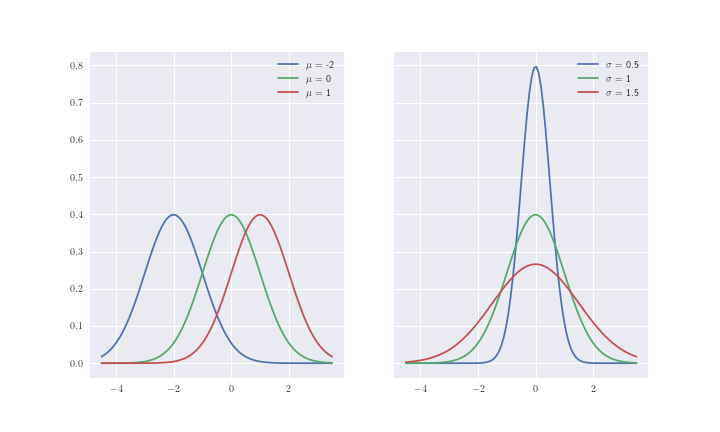
\includegraphics[scale = 0.45]{\pathtoimages/ex3-1.png}
\end{figure}

\end{frame}

\begin{frame}
\frametitle{Standard Normal Distribution}
\begin{Definition}
The {\bf standard normal distribution} is $\mathcal{N}(0, 1^2)$, i.e. it is a normal distribution with $\mu = 0$ and $\sigma^2 = 1$. The pdf and cdf are sometimes denoted $\phi$ and $\Phi$, respectively. 
\end{Definition}
You can translate a normal random variable into a standard normal variable by calculating its $Z$-score:
$$
X\sim{\mathcal{N}(\mu, \sigma^2)}\qquad\text{implied}\qquad Z = \frac{X - \mu}{\sigma}\sim{\mathcal{N}(0, 1^2)}.
$$
\end{frame}


\begin{frame}
\frametitle{Empirical Rule}
\small
\begin{center}
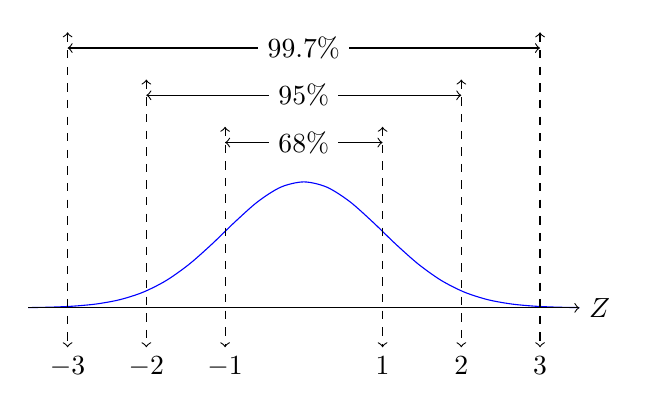
\begin{tikzpicture}[declare function = {normal(\x) = 1.6 * exp(-0.5 * \x * \x);}, ]
% Draw and label normal distribution function
\draw[color=blue, domain=-3.5:3.5, smooth] plot (\x, {normal(\x)});


\draw[->] (-3.5, 0) -- (3.5, 0) node[right] {$Z$};


\draw[dashed, <->] (-1, 2.3) -- (-1, -0.5) node[below] {$-1$};
\draw[dashed, <->] (1, 2.3) -- (1, -0.5) node[below] {$1$};

\draw[<->] (-1, 2.1) -- (1, 2.1);
\node[fill = white] at (0, 2.1) {$68\%$};


\draw[dashed, <->] (-2, 2.9) -- (-2, -0.5) node[below] {$-2$};
\draw[dashed, <->] (2, 2.9) -- (2, -0.5) node[below] {$2$};

\draw[<->] (-2, 2.7) -- (2, 2.7);
\node[fill = white] at (0, 2.7) {$95\%$};


\draw[dashed, <->] (-3, 3.5) -- (-3, -0.5) node[below] {$-3$};
\draw[dashed, <->] (3, 3.5) -- (3, -0.5) node[below] {$3$};

\draw[<->] (-3, 3.3) -- (3, 3.3);
\node[fill = white] at (0, 3.3) {$99.7\%$};

\end{tikzpicture}
\end{center}
If $Z\sim{\mathcal{N}(0, 1^2)}$, then
$$
P(|Z| < 1) \approx 68\%,\qquad P(|Z| < 2) \approx 95\%,\qquad\text{and}\qquad P(|Z| < 3) = 99.7\%.
$$
\end{frame}

\begin{frame}[t]
\frametitle{Normal Distribution Example}
\begin{Example}
Suppose that the daily returns for a stock index $R\sim{\mathcal{N}{(0, 0.01^2)}}$. What is the probability of this index dropping more than 3\%?
\end{Example}

\end{frame}

\begin{frame}
\frametitle{Exponential Distribution}
\small
\begin{Definition}
The {\bf exponential distribution} describes an experiment where events occur continuously and independently at a constant average rate $\lambda$. Exponential random variables are often used to model arrival times, waiting
times, and equipment failure times.
\end{Definition}
To denote that the random variable $X$ follows and exponential distribution, we write $X\sim{\mathcal{E}(\lambda)}$. The pdf and cdf of an exponential distribution are
$$
f(x) = \begin{cases} 0, & x < 0\\ \lambda e^{-\lambda x},& x\geq 0\end{cases} \qquad\text{and}\qquad F(x) = \begin{cases} 0,	&	x < 0\\ 1 - e^{-\lambda x},&	x\geq 0.\end{cases}
$$

\end{frame}

\begin{frame}[t]
\frametitle{Exponential Distribution Example}
\begin{Example}
Suppose that the time until default, measured in years, of a firm $T$ follows an exponential distribution with $\lambda = 0.10$. What is the probability that $2 < T < 5$?
\end{Example}

\end{frame}

\subsection{Expected Values}

\begin{frame}
\frametitle{Expected Values}
\begin{Definition}
The {\bf expected value} of a discrete random variable $X$ is
$$
E[X] = \mu_X = \sum_x xP(x),
$$
where we sum over the range of $X$. If $X$ is a continuous random variable, then the expected value is
$$
E[X] = \mu_X = \int_{-\infty}^\infty x f(x)\ dx.
$$
\end{Definition}
\end{frame}

\begin{frame}
\frametitle{Property of Expected Values}
For random variables $X$ and $Y$, and scalars $\alpha$ and $\beta$, we have
$$
E[\alpha X + \beta Y] = \alpha E[X] + \beta E[Y].
$$
\end{frame}

\begin{frame}[t]
\frametitle{Expected Values Example}
\begin{Example}
Suppose that the pmf of $N$ is
$$
p(n) = \begin{cases} \left(\frac{1}{2}\right)^n,	&	n = 1, 2 ,\ldots\\ 0,	&\text{otherwise.}\end{cases}
$$
Calculate $E[N]$.
\end{Example}
\end{frame}


\begin{frame}
\frametitle{Variance and Standard Deviation}
\begin{Definition}
The {\bf variance} of a discrete random variable $X$ is
$$
\text{Var}(X) = \sigma_X^2 = \sum_x \left(x - \mu_X \right)^2 p(x).
$$
If $X$ is a continuous random variable
$$
\text{Var}(X) = \sigma_X^2 = \int_{-\infty}^\infty \left(x - \mu_X\right)^2 f(x)\ dx.
$$
The {\bf standard deviation} of $X$ is the square root of its variance and is denoted by $\sigma_X$.
\end{Definition}
\end{frame}

\begin{frame}[t]
\frametitle{Variance Example}
\begin{Example}
Prove the identity 
$$
\text{Var}(X) = E[X^2] - \left(E[X]\right)^2.
$$
\end{Example}
\end{frame}

\begin{frame}
\frametitle{Property of Variance}
For random variable $X$ and scalars $\alpha$ and $\beta$
$$
\text{Var}\left(\alpha X + \beta\right) = \alpha^2 \text{Var}(X).
$$
\end{frame}

\begin{frame}
\frametitle{Expected Value and Variance Formulas}

\begin{tabular}{ | c |	c	c | }
\hline
\text{Distribution}			&	\text{Expected Value}					&	\text{Variance}\\\hline
						&										&				\\
Discrete Uniform			&	$\displaystyle\frac{1}{n} \sum_{k = 1}^n x_k$	&	$\displaystyle\frac{1}{n} \sum_{k = 1}^n x_k^2 - \left(\frac{1}{n} \sum_{k = 1}^n x_k\right)^2$\\
$\mathcal{B}(n, p)$			&	$np$									&	$np(1 - p)$\\
$\mathcal{P}(\lambda)$		&	$\lambda$								&	$\lambda$\\
$\mathcal{U}(a, b)$			&	$\displaystyle\frac{b + a}{2}$				&	$\displaystyle\frac{(b - a)^2}{12}$		\\
$\mathcal{N}(\mu, \sigma^2)$	&	$\mu$								&	$\sigma^2$						\\
$\mathcal{E}(\lambda)$		&	$\displaystyle\frac{1}{\lambda}$				&	$\displaystyle\frac{1}{\lambda^2}$		\\
						&										&									\\\hline
\end{tabular}

\end{frame}

\subsection{Moments}

\begin{frame}
\frametitle{$k$-th Moment}
\begin{Definition}
\begin{itemize}
\item If $X$ is a random variable, then its $\boldsymbol k${\bf-th moment} is $E[X^k]$. 
\item If $\mu = E[X]$ and $\sigma^2 = \text{Var}(X)$, then the {\bf standardized} $\boldsymbol k${\bf-th moment} is $E\left[\left(\frac{X - \mu}{\sigma}\right)^k\right]$.
\end{itemize}
\end{Definition}
\end{frame}

\begin{frame}
\frametitle{Skew}
\begin{Definition}
The standardized third moment is the {\bf skew}.
\end{Definition}
\begin{figure}
\centering
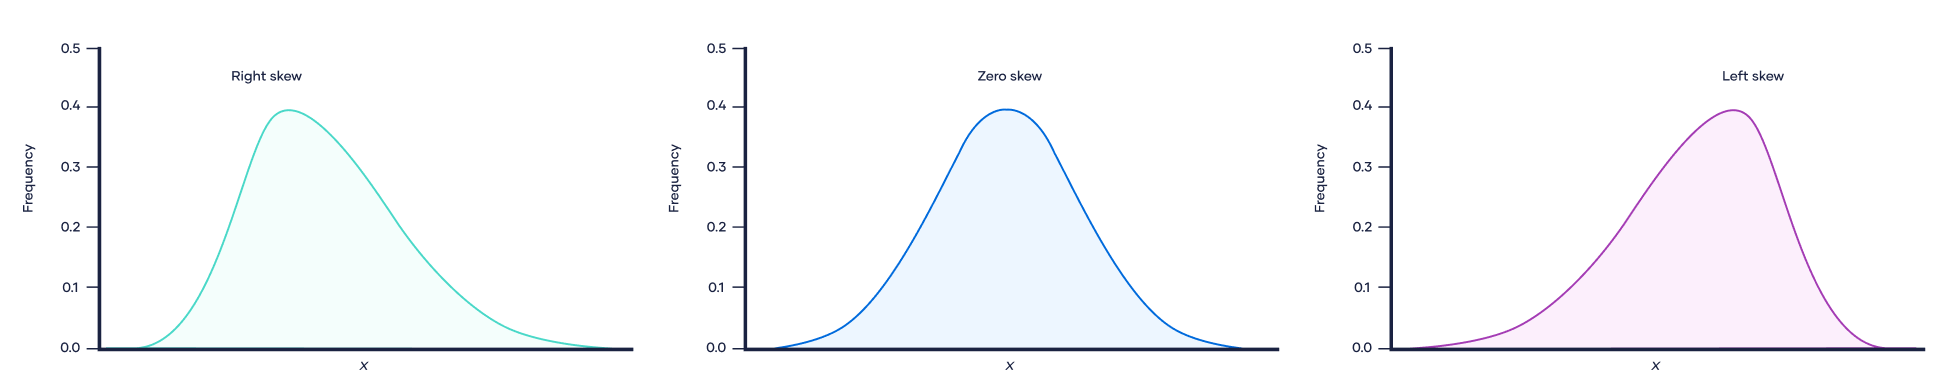
\includegraphics[scale = 0.17]{\pathtoimages/skew.png}
\end{figure}

\end{frame}

\begin{frame}
\frametitle{Kurtosis}
\small
\begin{Definition}
The standardized fourth moment is the {\bf kurtosis}. A normal distribution has kurtosis of 3. If the kurtosis is greater than 3, it is {\bf leptokurtic}, and if the kurtosis is less than 3 it {\bf platykurtic}.
\end{Definition}
\begin{figure}
\centering
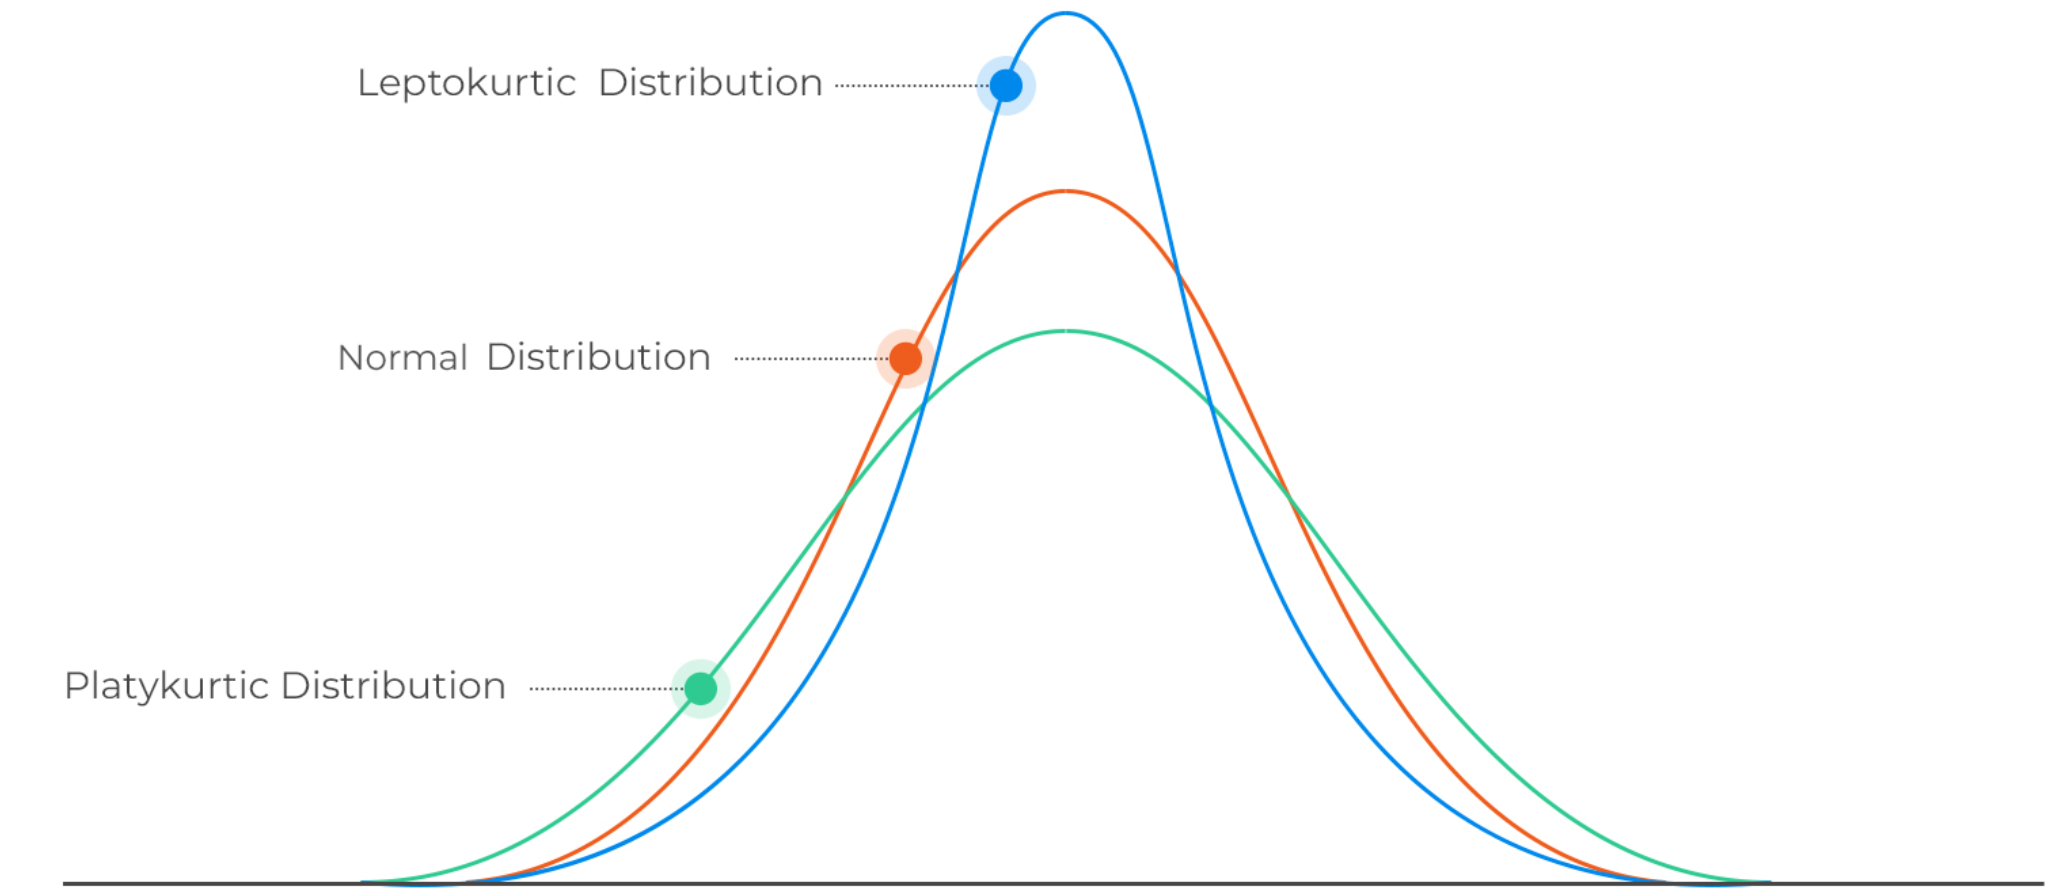
\includegraphics[scale = 0.13]{\pathtoimages/kurtosis.png}
\end{figure}
The kurtosis is typically considered a measure of tail thickness, though the true the meaning is more nuanced:
\begin{center}{\tiny\url{https://stats.stackexchange.com/questions/172467/what-is-the-meaning-of-tail-of-kurtosis}}.
\end{center}
\end{frame}



\begin{frame}
\frametitle{Moment Generating Function}
\begin{Definition}
The {\bf moment generating function} of a random variable $X$ is
$$
\psi(t) = E[e^{tX}].
$$
\end{Definition}
We call $\psi$ the moment generating function of $X$ because
$$
E[X^k] = \psi^{(k)}(0).
$$
To see why this is the case, it is helpful to note
$$
e^{tX} = 1 + tX + \frac{(tX)^2}{2!} + \frac{(tX)^3}{3!} + \ldots.
$$
\end{frame}

\begin{frame}[t]
\frametitle{Moment Generating Function Example}
\begin{Example}
Find the moment generating function of $X$, the discrete uniform distribution with support $\{1, 2, 3\}$.
\end{Example}

\end{frame}

\subsection{Functions of a Random Variable}

\begin{frame}[fragile]
\frametitle{Function of a RV Python Example}
\small
\begin{Example}
Suppose $Z\sim{\mathcal{N}(0, 1)}$. Consider $X = Z^2$. Use Python to approximate the graph of the pdf of $X$ using a histogram. 
\end{Example}

\begin{lstlisting}[language=Python]
# Import modules
import numpy as np, matplotlib.pyplot as plt
from scipy.stats import norm

# Use LaTeX
plt.rcParams['text.usetex'] = True

# Use Seaborn style
plt.style.use('seaborn')

# Generate Z
Z = norm.rvs(size = 100_000)

# Calculate X
X = Z**2

# Generate histogram; make sure density is True
plt.hist(X, bins = 100, density = True)

# Get title 
plt.title(r'Histogram of $X = Z^2$')

# Save the figure
plt.savefig(path + r'ex3-2.png')

plt.show()
\end{lstlisting}
\end{frame}

\begin{frame}
\frametitle{Function of a Random Variable Python Result}
\small 
This is a known distribution $\chi^2(1)$. See \href{https://en.wikipedia.org/wiki/Chi-squared_distribution}{Wikipedia} for more details. 
\begin{center}
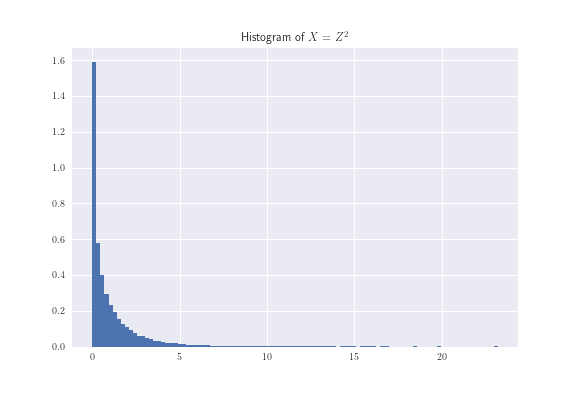
\includegraphics[scale = 0.40]{\pathtoimages/ex3-2.png}
\end{center}

\end{frame}

\begin{frame}
\frametitle{Functions of a Random Variable}
This result can be obtained analytically by considering the cdf and differentiating. 
\end{frame}

\begin{frame}[t]
\frametitle{Function of a Random Variable Example}
\begin{Example}
Suppose $Z\sim{\mathcal{N}(0, 1)}$. Consider $X = Z^2$. Calculate the pdf of $X$.
\end{Example}

\end{frame}

\begin{frame}
\frametitle{Functions of a Random Variable Theorem}

\begin{Theorem}
Let $X$ be a random variable with pdf $f$. Suppose $P(a < x < b) = 1$. Let $Y = r(X)$ and suppose $r$ is differentiable and one-to-one for $a < x < b$. Let the image of $(a, b)$ under $r$ be $(\alpha, \beta)$. If $s$ is the inverse of $r$, then the pdf of $Y$ is
$$
g(y) = \begin{cases} f\left(s(y)\right)\left|\frac{ds}{dy}\right|,	&	\alpha < y <\beta\\ 0,	&	\text{otherwise.}\end{cases}
$$
\end{Theorem}

\end{frame}

\begin{frame}[t]
\frametitle{Functions of a Random Variable Example}
\begin{Example}
Suppose $X\sim{\mathcal{U}(0, 1)}$ and let $Y = \frac{1}{27}X^3$. Find the pdf of $Y$.
\end{Example}

\end{frame}


\subsection{Joint Distributions} 

\begin{frame}

\frametitle{Joint Distributions}
\begin{Definition}
Two random variables $X$ and $Y$ are said to be {\bf jointly continuous} if there exists a function $f_{XY}(x, y) \geq 0$ with the property that for every subset $C$ of $\mathbb{R}^2$, we have
$$
P\Big((X, Y)\in C\Big) = \iint_C f_{XY}(x, y)\ dA.
$$
The function $f_{XY}(x, y)$ is called the {\bf joint probability density function} of $X$ and $Y$, and the {\bf joint cumulative distribution function} is
$$
F(x, y) = \int_{-\infty}^y\int_{-\infty}^x f(s, t)\ ds\,dt.
$$
\end{Definition}

\end{frame}

\begin{frame}[t]
\frametitle{Joint Distributions Example}
\begin{Example}
\small
Suppose
$$
f_{XY}(x, y) = \begin{cases} \frac{1}{2},	&	-1\leq x \leq y \leq 1\\ 0, &	\text{otherwise.}\end{cases}
$$
Then $P(2X - Y > 0) = $
\end{Example}
\end{frame}

\begin{frame}
\frametitle{Marginal PDF}
The marginal pdfs of $X$ and $Y$ given joint pdf $f_{XY}$ are
$$
f_X(x) = \int_{-\infty}^\infty f(x,y)\ dy\qquad\text{and}\qquad f_Y(y) = \int_{-\infty}^\infty f(x, y)\ dx.
$$
\end{frame}

\begin{frame}
\frametitle{Independent Events}
If the random variables $X$ and $Y$ are independent, then
$$
f_{XY}(x, y) = f_X(x) f_Y(y).
$$
\end{frame}

\begin{frame}[t]
\frametitle{Independent Events Example}
\small
\begin{Example}
The joint pdf of $X$ and $Y$ is given by
$$
f_{XY}(x, y) = \begin{cases} 3(x + y),&	x +y \leq 1, x,y \geq  0\\ 0, & \text{otherwise.}\end{cases}	
$$
Are $X$ and $Y$ independent? 
\end{Example}

\end{frame}

\begin{frame}
\frametitle{Change of Variables}
\tiny
\begin{Theorem}
Let $X$ and $Y$ be continuous random variables with joint density $f_{XY}$. Assume that there is a subset $S$ of $\mathbb{R}^2$ such that
$P\Big((X, Y)\in S\Big) = 1$. Let 
$$
U = r_1(X, Y)\qquad\text{and}\qquad V = r_2(X, Y),
$$ 
where $r_1$ and $r_2$ are one-to-one differentiable transformations from $S$ onto some subset $T$ of $\mathbb{R}^2$. If 
$$
X = s_1(U, V)\qquad\text{and}\qquad Y = s_2(U, V)
$$ 
describe the inverse transformation, where $s_1$ and $s_2$ are also one-to-one and differentiable. Then the joint pdf of $U$ and $V$ is
$$
g_{UV}(u, v) = \begin{cases} f_{XY}\Big(s_1(u, v), s_2(u, v)\Big)\left|\text{det}(J)\right|,	&	(u, v)\in T\\ 0,&	\text{otherwise.}\end{cases}
$$
where 
$$
J = \left(\begin{array}{c c} \dfrac{\partial s_1}{\partial u}	&	\dfrac{\partial s_1}{\partial v}\\ \dfrac{\partial s_2}{\partial u}	&	\dfrac{\partial s_2}{\partial v}\end{array}\right)
$$
is the Jacobian.
\end{Theorem}

\end{frame}

\begin{frame}[t]
\frametitle{Change of Variables Example}
\begin{Example}
Suppose $f_{XY}(x, y) = \frac{1}{2\pi} e^{-\frac{x^2 + y^2}{2}}$. Find the joint pdf of $r$ and $\theta$, where $x = r\cos\theta$ and $y=r\sin\theta$.
\end{Example}
\end{frame}

\subsection{Covariance}
\begin{frame}
\frametitle{Covariance}
\begin{Definition}
Let $X$ and $Y$ be random variables having finite means. Suppose $E[X] = \mu_X$ and $E[Y] = \mu_Y$. The {\bf covariance of $\boldsymbol X$ and $\boldsymbol Y$} is
$$
\text{Cov}(X, y) = E\Big[(X - \mu_X)(Y - \mu_Y)\Big].
$$
\end{Definition}
A useful identity is
$$
\text{Cov}(X, Y) = E[XY] - E[X]E[Y].
$$
\end{frame}

\begin{frame}[t]
\frametitle{Covariance Example 1}
\tiny
\begin{Example}
Consider $X$ and $Y$ with joint pdf
$$
f_{XY}(x, y) = \begin{cases} 2, &	0\leq x \leq y\leq 1\\ 0,	&	\text{otherwise.}\end{cases}
$$
Calculate the covariance of $X$ and $Y$. Hint: $E[X] = \frac{1}{3}$ and  $E[Y] =  \frac{2}{3}.$
\end{Example}

\end{frame}

\begin{frame}[t]
\frametitle{Covariance Example 2}
\begin{Example}
Suppose $X\sim{\mathcal{U}(-1, 1)}$. Calculate the covariance between $X$ and $X^2$.
\end{Example}

\end{frame}


\begin{frame}
\frametitle{Properties of Covariance}
Suppose $X_i$ and $Y_j$ are random variables for all $i$ and $j$, and $\alpha$ is a real number.
\begin{enumerate}
\item[(a)] $\text{Cov}(X_1, X_2) = \text{Cov}(X_2, X_1)$
\item[(b)] $\text{Cov}(X_1, X_1) = \text{Var}(X_1)$
\item[(c)] $\text{Cov}(\alpha X_1, X_2) = \alpha \text{Cov}(X_1, X_2)$
\item[(d)] $\text{Cov}(X,Y) = 0$ if $X$ and $Y$ are independent 
\item[(e)] $\displaystyle \text{Cov}\left(\sum_{i = 1}^m X_i, \sum_{j = 1}^n Y_j\right) = \sum_{i = 1}^m\sum_{j = 1}^n \text{Cov}(X_i, Y_j)$
\end{enumerate}

\end{frame}

\begin{frame}
\frametitle{Correlation}
\begin{Definition} 
Let $X$ and $Y$ be random variables with finite variances $\sigma_X^2$ and $\sigma_Y^2$, respectively. Then the {\bf correlation of $\boldsymbol X$ and $\boldsymbol Y$} is
$$
\rho(X, Y) = \frac{\text{Cov}(X, Y)}{\sigma_X\sigma_Y}.
$$
\end{Definition}
In Python the correlation between two variables can be calculated using \texttt{np.corrcoef}. See the \href{https://numpy.org/doc/stable/reference/generated/numpy.corrcoef.html}{NumPy documentation} for more details.
\end{frame}

\begin{frame}[fragile]
\frametitle{Correlation Plot Python Code}
\begin{multicols}{2}
\begin{lstlisting}[language=Python]
# Import modules
import numpy as np, matplotlib.pyplot as plt
from scipy.stats import norm

# Use LaTeX
plt.rcParams['text.usetex'] = True

# Use Seaborn style
plt.style.use('seaborn')

# Generate standard normals
Z = norm.rvs(size = 100)

# List correlations
rho_vals = [-0.9, -0.75, -0.25, 0.25, 0.75, 0.9]

# Set up subplots
fig, ax = plt.subplots(2, 3, sharey = True, 
                       figsize = (12, 10), dpi = 125)

for i, rho in enumerate(rho_vals):
    
    # Get X and Y values
    X = np.linspace(0, 1, len(Z))
    Y = rho * X + np.sqrt(1 - rho**2) * Z
    
    # Get row and column
    row, col = i//3, i%3
    
    # Draw scatter plot
    ax[row, col].scatter(X, Y)
    
    # Draw plot of underlying relationship
    ax[row, col].plot(X, rho * X, color = 'red')
    
    # Add title to subplot
    ax[row, col].set_title(r'$\rho =$ ' + str(rho))
    
    # Add labels for x and y axes
    ax[row, col].set_xlabel(r'$X$')
    ax[row, col].set_ylabel(r'$Y$')
    
# Save the figure
plt.savefig(path + r'ex3-3.png')

plt.show()
\end{lstlisting}
\end{multicols}
\end{frame}

\begin{frame}[fragile]
\frametitle{Correlation Plot}
\begin{figure}
\centering
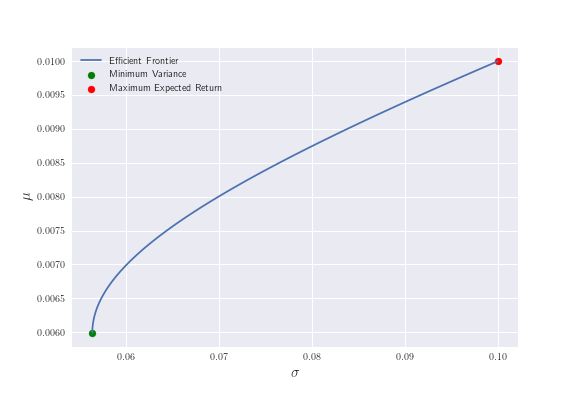
\includegraphics[scale = 0.3]{\pathtoimages/ex3-3.png}
\end{figure}

\end{frame}


\begin{frame}
\frametitle{Variance of Sum}

\begin{Theorem}
If $X$ and $Y$ are random variables and $\alpha$ and $\beta$ are constants, then
$$
\text{Var}(\alpha X + \beta Y) = \alpha^2 \text{Var}(X) + \beta^2\text{Var}(Y) + 2\alpha\beta \text{Cov}(X, Y).
$$
\end{Theorem}
\end{frame}

\begin{frame}[t]
\frametitle{Variance of Sum Example}
\begin{Example}
Suppose $X\sim{\mathcal{U}(-1, 1)}$. Calculate the variance of $X - 2 X^2$.
\end{Example}

\end{frame}

\subsection{Efficient Frontier}

\begin{frame}
\frametitle{Efficient Frontier}

\begin{Definition}
The {\bf efficient frontier} is the set of portfolios which satisfy the condition that no other portfolio in the investment universe exists with a higher expected return and the same standard deviation of return.
\end{Definition}
\begin{figure}
\centering
\begin{tikzpicture}[scale = 0.75]

\draw[->] (-1, -0.5) -- (-1, 3.5) node[above] {\text{Expected Return}};
\draw[->] (-1, -0.5) -- (4, -0.5) node[right] {\text{Standard Deviation}};

\draw[domain=0:2, smooth, variable=\y, blue, ->]  plot ({\y*\y}, {\y});

\node[green] at (0, 0) {$\bullet$};

\end{tikzpicture}
\end{figure}
\end{frame}

\begin{frame}
\frametitle{Portfolio Construction}
\begin{Example}
Consider assets 1 and 2 with monthly expected returns of 1\% and 0.5\% and standard deviations of 10\% and 6\%, respectively. Suppose the correlation between returns is 25\%.
\begin{enumerate}
\item[(a)] Find the minimum variance portfolio.
\item[(b)] Graph the efficient frontier.
\end{enumerate}
Assume that you cannot take short positions in this investment universe.
\end{Example}

\end{frame}

\begin{frame}[fragile]
\frametitle{Portfolio Construction Python Code}

\begin{lstlisting}[language=Python]
# Import modules
import numpy as np, pandas as pd, matplotlib.pyplot as plt
from scipy.optimize import minimize_scalar

# Use LaTeX
plt.rcParams['text.usetex'] = True

# Use Seaborn style
plt.style.use('seaborn')

# Define expected returns
mu1, mu2 = 0.01, 0.005

# Define standard deviations
sigma1, sigma2 = 0.10, 0.06

# Define correlation
rho = 0.25

# Create function for portfolio expected return
def port_mu(w):
    
    return mu1 * w + mu2 * (1 - w)

# Create function for portfolio standard deviations
def port_sigma(w):
    
    # Calculate variance...
    
    # ... uncorrelated variance
    var = w**2 * sigma1**2 + (1 - w)**2 * sigma2**2 
    
    # ... variance due to correlation
    var +=  2 * w * (1 - w) * rho * sigma1 * sigma2
    
    # Take square root to obtain standard deviation
    return np.sqrt(var)
\end{lstlisting}

\end{frame}


\begin{frame}[fragile]
\frametitle{Portfolio Construction Python Code}

\begin{lstlisting}[language=Python]
# Get weights for minimum variance portfolio; no short positions
w_min_var = minimize_scalar(port_sigma, bounds = (0, 1), method = 'bounded').x
                            
# Define number of samples
samples = 100

# Create data frame to save results
port_results = pd.DataFrame(index = range(samples), columns = ['mu', 'sigma'])

# Get weights to loop over
wt_vals = np.linspace(w_min_var, 1.0, samples)

# Calculate efficient frontier
for i, w in enumerate(wt_vals):
    
    # Calculate expected return
    mu = port_mu(w)
    
    # Calculate standard deviation
    sigma = port_sigma(w)
    
    # Save results
    port_results.loc[i, ['mu', 'sigma']] = mu, sigma
\end{lstlisting}

\end{frame}

\begin{frame}[fragile]
\frametitle{Portfolio Construction Python Code}

\begin{lstlisting}[language=Python]
# Plot efficient frontier
plt.plot(port_results['sigma'], port_results['mu'], label = 'Efficient Frontier')

# Add dot for minimum variance portfolio
plt.scatter(port_results.loc[0, 'sigma'], port_results.loc[0, 'mu'], label = 'Minimum Variance', color = 'green')

# Add dot for maximum expected return
plt.scatter(port_results.loc[samples - 1, 'sigma'], port_results.loc[samples - 1, 'mu'], 
            label = 'Maximum Expected Return', color = 'red')

# Add legend
plt.legend()

# Add x-label
plt.xlabel(r'$\sigma$', fontsize = 15)

# Add y-label
plt.ylabel(r'$\mu$', fontsize = 15)

# Save the figure
plt.savefig(path + r'ex3-4.png')

plt.show()

print(r'The minimum variance portfolio has respective weights in', 
      r'assets 1 and 2 of', 
      f'{100 * w_min_var:.1f}% and {100 - 100 * w_min_var:.1f}%.',
     f'The standard deviation of the minimum variance portfolio is {100 * port_sigma(w_min_var):.1f}%.')
      \end{lstlisting}

\end{frame}


\begin{frame}
\frametitle{Portfolio Construction Result}
The minimum variance portfolio has respective weights in assets 1 and 2 of 19.8\% and 80.2\%. The standard deviation of the minimum variance portfolio is 5.6\%.
\begin{figure}
\centering
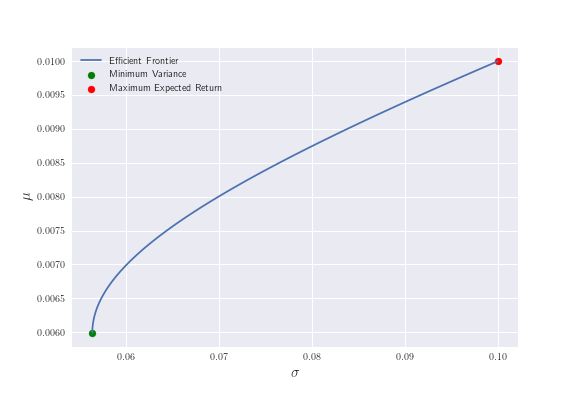
\includegraphics[scale = 0.4]{\pathtoimages/ex3-4.png}
\end{figure}
\end{frame}

\section{Statistics}



\subsection{Inequalities} 

\begin{frame}
\frametitle{Markov Inequity}

\begin{Theorem}[Markov Inequity] 
Suppose $X$ is a random variable such that $P(X\geq 0) = 1$. Then for each real number $t > 0$,
$$
P(X\geq t) \leq \frac{E[X]}{t}.
$$
\end{Theorem}
\end{frame}

\begin{frame}
\frametitle{Chebyshev Inequality}

\begin{Theorem}[Chebyshev Inequality]
Let $X$ be a random variable for which $\text{Var}(X)$ exists. Then for every number $t > 0$,
$$
P\Big(\left| X - E[X]\right| \geq t\Big) \leq \frac{\text{Var}(X)}{t^2}.
$$
\end{Theorem}

\end{frame}

\frametitle{Sampling} 

\begin{frame}
\frametitle{Mean and Variance of Sample Mean}

\begin{Theorem}
Let $X_1, X_2,\ldots, X_n$ be an independent random sample from a distribution with mean $\mu$ and variance $\sigma^2$. Let $\bar{X}_n$ be the sample mean. Then $E[\bar{X}_n] = \mu$ and $\text{Var}(\bar{X}_n) =\frac{\sigma^2}{n}$.
\end{Theorem}
\end{frame}

\begin{frame}[t]
\frametitle{Mean and Variance of Sample Mean}
\begin{Example}
Suppose $E[X] = 0$ and $\text{Var}(X) = 1$. Use Chebyshev Inequality to find a minimum value of $n$, so that $P\Big(|\bar{X}_n| \geq 0.5\Big) \leq 0.01$?
\end{Example}

\end{frame}


\subsection{Law of Large Numbers}

\begin{frame}
\frametitle{Convergence in Probability}
\begin{Definition}
A sequence $X_1, X_2,\ldots$ of random variables {\bf converges in probability} to $b$ if for each $\epsilon > 0$,
$$
\lim_{n\to\infty} P\Big(|X_n - b| < \epsilon\Big) = 1.
$$
\end{Definition}
We often write $X_n\stackrel{p}{\longrightarrow} b$ to denote that the sequence converges in probability to $b$.
\end{frame}

\begin{frame}
\frametitle{Law of Large Numbers}

\begin{Theorem}[Law of Large Numbers]
Suppose that $X_1, X_2,\ldots, X_n$ form a random sample from a distribution with mean $\mu$ and finite variance. Let $\bar{X}_n$ denote the sample mean. Then
$$
\bar{X}_n\stackrel{p}{\longrightarrow} \mu.
$$
\end{Theorem}

\end{frame}

\begin{frame}[t]
\frametitle{Law of Large Numbers Example}
\begin{Example}
\small
Use an exponential distribution with $\lambda = 1$ to illustrate the Law of Large Numbers. Generate 100,000 samples each of size $n$, for $n = 100, 500, 1000,$ and $10,000$.
\end{Example}

\end{frame}

\begin{frame}[fragile]
\frametitle{Law of Large Numbers Example Python Code}

\begin{lstlisting}[language=Python]
# Import modules
import numpy as np, matplotlib.pyplot as plt, time
from scipy.stats import expon

# Start the clock!
start_time = time.perf_counter()

# Set random seed
np.random.seed(0)

# Use LaTeX and Seaborn style
plt.rcParams['text.usetex'] = True
plt.style.use('seaborn')

# Choose n-values and set number of trials
n_vals, trials = [100, 500, 1000, 10_000], 100_000

# Set up subplots
fig, ax = plt.subplots(1, 4, sharex = True, sharey = True, 
                       figsize = (12, 4), dpi = 125)
for i, n in enumerate(n_vals):
    
    # Generate numbers of dimension trails x n
    # Scale is 1/lambda; default is 1 so unnecessary
    X = expon.rvs(scale = 1/1, size = (trials, n))
         
    # Take mean of each row and make histogram
    ax[i].hist(X.mean(axis = 1), bins = int(np.log(n)), density = True)
    ax[i].vlines(x = 1, ymin = 0, ymax = 35, linestyle = 'dashed', 
                 color = 'red', label = 'True Mean')
    
    # Give each histogram a title
    ax[i].title.set_text(f'$n = {n}$')
    
    # Add legend
    ax[i].legend()
\end{lstlisting}
\end{frame}

\begin{frame}[fragile]
\frametitle{Law of Large Numbers Example Python Code}

\begin{lstlisting}[language=Python]
# Clear up a little RAM
del X

# Give the entire figure a title
fig.suptitle('Law of Large Numbers Using Exponential Distribution')

# Save the figure
plt.savefig(path + r'ex3-5.png')

plt.plot()

# When my programs run slowly, I like to monitor the time it takes
print(f'This program took {time.perf_counter() - start_time:.3f} seconds.')
\end{lstlisting}
\end{frame}


\begin{frame}
\frametitle{Law of Large Numbers Result}
\begin{figure}
\centering
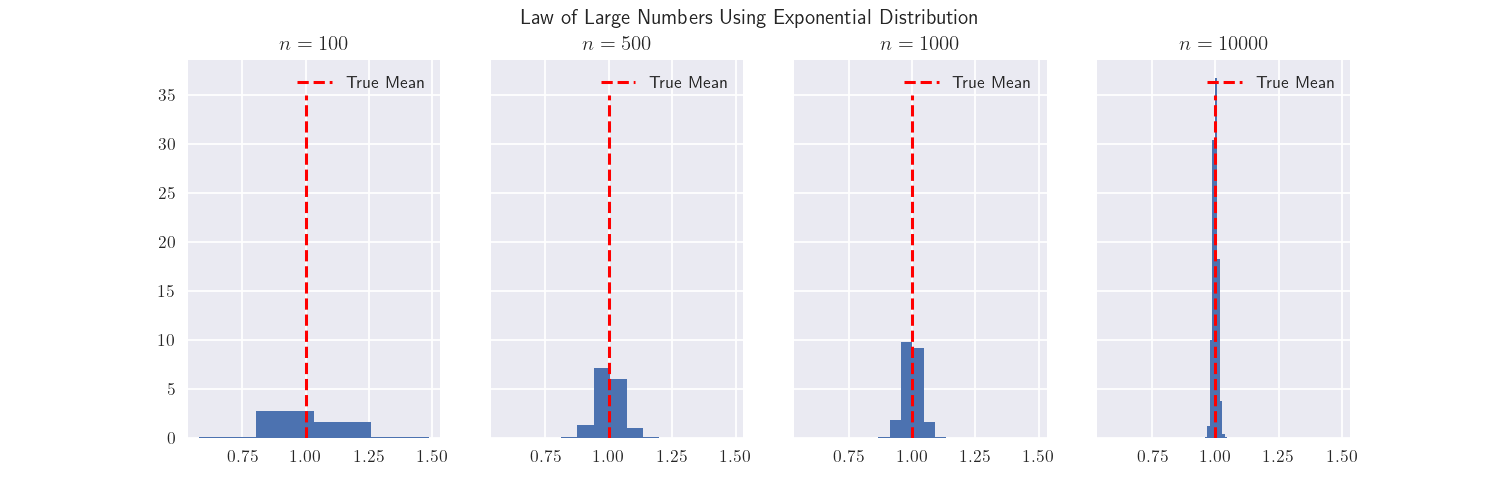
\includegraphics[scale = 0.40]{\pathtoimages/ex3-5.png}
\end{figure}
\end{frame}

\begin{frame}
\frametitle{Convergence in Distribution}
\begin{Definition}
A sequence $X_1, X_2,\ldots$ of random variables with cdfs $F_1, F_2,\ldots$ {\bf converge in distribution} to the random variable $X$ with cdf $F$ if
$$
\lim_{n\to\infty} F_n(x) = F(x)
$$
for every number $x$ at which $F$ is continuous. 
\end{Definition}
We often write $X_n \stackrel{d}{\longrightarrow} X$ to denote converges in distribution.
\end{frame}

\subsection{Empirical CDFs}

\begin{frame}
\frametitle{Empirical CDFs}
\small
\begin{Definition}
Suppose we have observed data $x_1, x_2, \ldots, x_n$ which are sampled from the same distribution. The empirical cdf given these data is
$$
F_n(x) = \frac{1}{n} \sum_{k = 1}^n {\bf 1}_k (x),
$$
where
$$
 {\bf 1}_k(x) = \begin{cases} 1,	&	x _k\leq x\\ 0,&	\text{otherwise.}\end{cases}
$$
\end{Definition}
In Python, it's very easy to code the empirical cdf:
\begin{center} 
\texttt{ecdf = lambda x, data: np.mean(data <= x)}.
\end{center}
\end{frame}

\begin{frame}[fragile]
\frametitle{Empirical CDFs Python Example}
\small
\begin{Example}
Graph the empirical cdf of a $\chi^2(1)$ distribution with a sample of size 5, 50, and 1000 as well as the true cdf of the $\chi^2(1)$.
\end{Example}

\begin{lstlisting}[language=Python]
# Import modules
import numpy as np, matplotlib.pyplot as plt
from scipy.stats import chi2

# Use LaTeX
plt.rcParams['text.usetex'] = True

# Use Seaborn style
plt.style.use('seaborn')

# Set random seed
np.random.seed(0)

# Create empirical cdf
ecdf = lambda x, data: np.mean(data <= x)

# List of sample sizes
sample_sizes = [5, 50, 1000]

# Create x-values for plot
x_vals = np.linspace(0, 5, 500)
\end{lstlisting}

\end{frame}

\begin{frame}[fragile]
\frametitle{Empirical CDFs Python Example}

\begin{lstlisting}[language=Python]
# Loop over the sample sizes
for sample_size in sample_sizes:
    
    # Generate data
    data = chi2.rvs(df = 1, size = sample_size)
    
    # Get the y-values
    y_vals = [ecdf(x, data) for x in x_vals]
    
    # Plot values
    plt.plot(x_vals, y_vals, label = f'size = {sample_size}')

# Get y-values; function vectorized
y_vals = chi2.cdf(x_vals, df = 1)

# Plot standard normal cdf
plt.plot(x_vals, y_vals, label = f'$\chi^2$')

# Clear up RAM
del data, x_vals, y_vals

# Show legend
plt.legend()

# Save the figure
plt.savefig(path + r'ex3-6.png')

plt.show()
\end{lstlisting}

\end{frame}

\begin{frame}[fragile]
\frametitle{Empirical CDFs Python Result}
\begin{center}
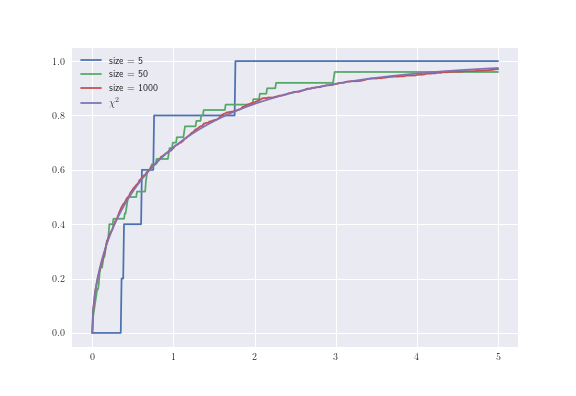
\includegraphics[scale = 0.4]{\pathtoimages/ex3-6.png}
\end{center}

\end{frame}

\subsection{Central Limit Theorem}

\begin{frame}
\frametitle{Central Limit Theorem}

\begin{Theorem}[Central Limit Theorem]
If the random variables $X_1, X_2, \ldots, X_n$ are a random independent sample of size $n$ from a given distribution with mean $\mu$ and finite variance $\sigma^2$, then
$$
\frac{\sqrt{n}}{\sigma}\left(\bar{X}_n - \mu\right)\stackrel{d}{\longrightarrow} \mathcal{N}(0, 1).
$$
\end{Theorem}
In other words, the sample mean should approximately follow the the distribution $\mathcal{N}\left(\mu, \frac{\sigma^2}{n}\right)$ when $n$ is large.
\end{frame}

\begin{frame}[t]
\frametitle{Central Limit Theorem Python Example}
\begin{Example}
Illustrate the Central Limit Theorem with an exponential distribution, using the empirical cdf and means of samples of size 2, 5, and 100.
\end{Example}

\end{frame}

\begin{frame}[fragile]
\frametitle{Central Limit Theorem Python Code}
\begin{lstlisting}[language=Python]
# Import modules
import numpy as np, matplotlib.pyplot as plt
from scipy.stats import expon, norm

# Use LaTeX
plt.rcParams['text.usetex'] = True

# Use Seaborn style
plt.style.use('seaborn')

# Set random seed
np.random.seed(0)

# Create empirical cdf
ecdf = lambda x, data: np.mean(data <= x)

# Create x-values for plot
x_vals = np.linspace(-5, 5, 500)

# Create n_values
n_vals = [2, 5, 100]

# Let's do 100,000 samples
samples = 100_000
\end{lstlisting}

\end{frame}

\begin{frame}[fragile]
\frametitle{Central Limit Theorem Python Code}
\begin{lstlisting}[language=Python]
# Scale is 1/lambda
lam = 1

# Loop over the n-values
for n in n_vals:
    
    # Generate the data; mean is 1/lam and std is 1/lam
    data =  expon.rvs(scale = 1/lam, size = (samples, n)).mean(axis = 1)
    
    # Change data so it has mean 0 and sd 1; current mean 1/lam and sd 1/(lam * sqrt(n))
    data = np.sqrt(n)/(1/lam) * (data - 1/lam)
    
    # Get y-values
    y_vals = [ecdf(x, data) for x in x_vals]
    
    # Plot values
    plt.plot(x_vals, y_vals, label = f'$n =$ {n}')

# Get y-values
y_vals = norm.cdf(x_vals)

# Plot standard normal cdf
plt.plot(x_vals, y_vals, label = 'Normal')

# Show legend
plt.legend()

# Save the figure
plt.savefig(path + r'ex3-7.png')

plt.show()\end{lstlisting}

\end{frame}

\begin{frame}
\frametitle{Central Limit Theorem Python Result}
\begin{figure}
\centering
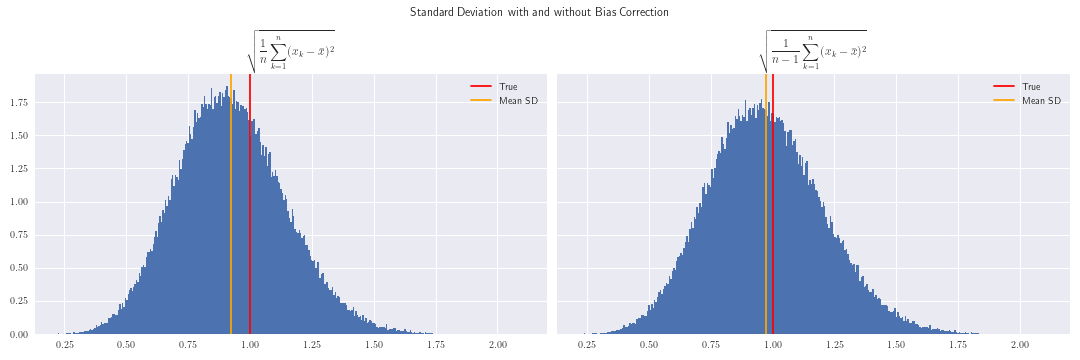
\includegraphics[scale = 0.4]{\pathtoimages/ex3-7.png}
\end{figure}

\end{frame}

\begin{frame}[t]
\frametitle{Central Limit Theorem Example}
\tiny
\begin{Example}
Assume that the weights of individuals are independent and normally distributed with a mean of 160 pounds and a standard deviation of 30 pounds. Suppose that twenty-five people squeeze into an elevator that is designed to hold 4300 pounds. What is the probability that the total weight exceeds the limit?
\end{Example}
\end{frame}

\begin{frame}
\frametitle{Central Limit Theorem on YouTube}
\small
3Blue1Brown has a great video on the Central Limit Theorem (\url{https://youtu.be/zeJD6dqJ5lo})
\begin{center}

\includegraphics[scale = 0.25]{\pathtoimages/central.png}
\end{center}
\end{frame}

\subsection{Hypothesis Testing}

\begin{frame}[t]
\frametitle{Hypothesis Testing Example}
\tiny
\begin{Example}
You sample the numbers 8, 0.5, 0, and $-0.5$ from a normal distribution with known variance of 1. Perform a hypothesis test to determine whether the mean of the distribution is statistically different from 0 at a significance level of 5\%.
\end{Example}

\end{frame}

\begin{frame}
\frametitle{Hypothesis Testing Steps}
\begin{enumerate}
\item State the hypotheses.
\item Set the criteria for a decision.
\item Compute the test statistic.
\item Make a decision.
\end{enumerate}
\end{frame}

\begin{frame}
\frametitle{State the Hypotheses}

\begin{Definition}
\begin{itemize}
\item The {\bf null hypothesis} ($H_0$) is a statement about a population parameter that is assumed to be true. We will test whether the value
stated in the null hypothesis is likely to be true.
\item An {\bf alternative hypothesis} ($H_1$) is a statement that directly contradicts the null hypothesis by stating that that the actual value of a population parameter is
less than, greater than, or not equal to the value stated in the null hypothesis.
\end{itemize}
\end{Definition}

\end{frame}

\begin{frame}
\frametitle{Set the Criteria for a Decision}

\begin{Definition}
{\bf Significance level} ($\alpha$) is a probability which denotes how strong the evidence must be before you reject the null hypothesis and conclude that the effect is statistically significant. 
\end{Definition}
\end{frame}

\begin{frame}
\frametitle{Hypothesis test for $H_0: \mu = \mu_0$}


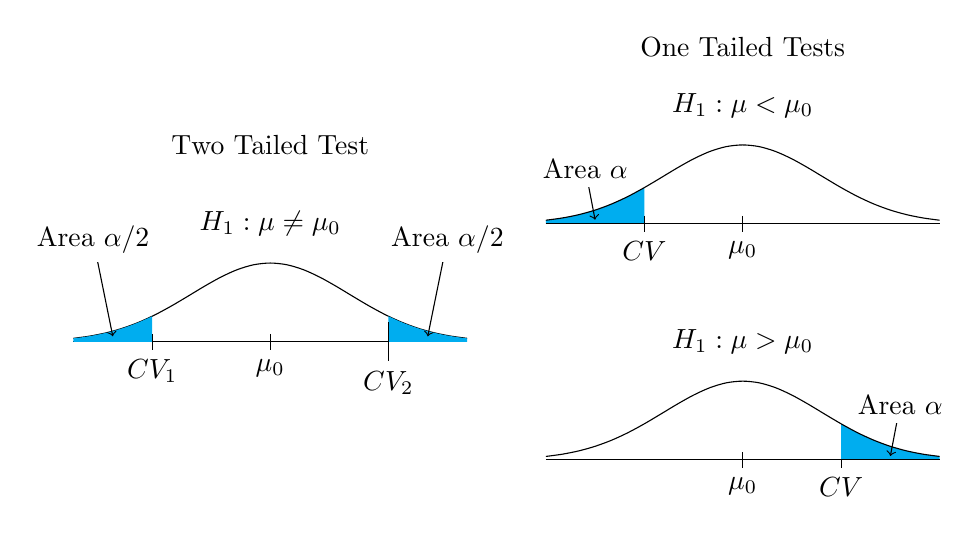
\begin{tikzpicture}

\node at (-3, 2.5) {Two Tailed Test};
\node at (-3, 1.5) {$H_1: \mu \neq \mu_0$};
\draw (-5.5, 0) -- (-0.5, 0);
\draw[domain=-2.5:2.5, smooth, variable=\x] plot ({\x - 3)}, {exp(-0.5 * \x * \x)});
\draw (-3, 0.10) -- (-3, -0.10) node[below] {$\mu_0$};

\fill[cyan, domain=-2.5:-1.5, variable=\x] (-5.5, 0) -- plot ({\x - 3},  {exp(-0.5 * \x * \x)}) -- (-4.5, 0) -- cycle;
\draw (-4.5, 0.10) -- (-4.5, -0.10) node[below] {$CV_1$};

\fill[cyan, domain=1.5:2.5, variable=\x] (-1.5, 0) -- plot ({\x - 3},  {exp(-0.5 * \x * \x)}) -- (-0.5, 0) -- cycle;
\draw (-1.5, 0.25) -- (-1.5, -0.25) node[below] {$CV_2$};


\draw[<-] (-1, 0.07) -- (-0.75, 1.3) node[fill = white] {Area $\alpha/2$};
\draw[<-] (-5, 0.07) -- (-5.25, 1.3) node[fill = white] {Area $\alpha/2$};

\node at (3, 3.75) {One Tailed Tests};

\node at (3, 3) {$H_1: \mu < \mu_0$};
\fill[cyan, domain=-2.5:-1.25, variable=\x] (0.5, 1.5) -- plot ({\x + 3},  {exp(-0.5 * \x * \x) + 1.5}) -- (1.75, 1.5) -- cycle;
\draw[domain=-2.5:2.5, smooth, variable=\x] plot ({\x + 3)}, {exp(-0.5 * \x * \x) + 1.5});
\draw (0.5, 1.5) -- (5.5, 1.5);
\draw (3, 1.6) -- (3, 1.4) node[below] {$\mu_0$};
\draw[<-] (1.125, 1.55) -- (1, 2.2) node[fill = white] {Area $\alpha$};

\draw (1.75, 1.60) -- (1.75, 1.4) node[below] {$CV$};

\node at (3, 0) {$H_1: \mu > \mu_0$};

\fill[cyan, domain=1.25:2.5, variable=\x] (4.25, -1.5) -- plot ({\x + 3},  {exp(-0.5 * \x * \x) - 1.5}) -- (5.5, -1.5) -- cycle;
\draw[domain=-2.5:2.5, smooth, variable=\x] plot ({\x + 3)}, {exp(-0.5 * \x * \x) - 1.5}); 
\draw (3, -1.4) -- (3, -1.6) node[below] {$\mu_0$};
 \draw (0.5, -1.5) -- (5.5, -1.5);
 \draw (4.25, -1.5) -- (4.25, -1.6) node[below] {$CV$};
\draw[<-] (4.875, -1.45) -- (5, -0.8) node[fill = white] {Area $\alpha$}; 

  
\end{tikzpicture}


\end{frame}

\begin{frame}
\frametitle{Compute the Test Statistic}
\begin{Definition}
A {\bf test statistic} quantifies the observed data in a way that would distinguish the null from the alternative hypothesis.
\end{Definition}

\end{frame}

\begin{frame}
\frametitle{Make a Decision}
\begin{Definition}
The $\boldsymbol p${\bf -value} is the probability of an observation being at least as extreme as the test statistic assuming the null hypothesis is true.
\end{Definition}

\end{frame}

\begin{frame}
\frametitle{Make a Decision Cont.}
\begin{itemize}
\item If the $p$-value is greater than or equal to $\alpha$, we {\it fail to reject the null hypothesis}.
\item If the $p$-value is less than $\alpha$, we {\it reject the null hypothesis}.
\end{itemize}
\end{frame}

\begin{frame}
\frametitle{Types of Error}
\begin{center}
\begin{tabular}{ c | c | c c }
							&						&	\multicolumn{2}{c}{Decision}		\\ \hline
							&						&	Fail to Reject Null	&	Reject Null	\\\hline
\multirow{4}{*}{Ground Truth}		&	\multirow{2}{*}{Null True}	&	Correct			&	Type I Error	\\
							&						&	$1 - \alpha$		&	$\alpha$		\\
							&	\multirow{2}{*}{Null False}	&	Type II Error		&	Correct		\\
							&						&	$\beta$			&	$1 - \beta$	\\		
\end{tabular}
\end{center}

\end{frame}

\begin{frame}
\frametitle{Confidence and Power}
\begin{Definition}
\begin{itemize}
\item The {\bf confidence level} is $1-\alpha$.
\item The {\bf power} is $1 - \beta$.
\end{itemize}
\end{Definition}
\end{frame}


\begin{frame}
\frametitle{Types of Hypothesis Tests}
\small
Incomplete list of types of hypothesis tests.

\begin{tabular}{p{1.3in} c p{2in}}
\hline
Name				&	Test Statistic							&	Comments \\\hline
One-sample $z$-test		&	$z = \frac{\bar{X} - \mu_0}{\sigma/\sqrt{n}}$	&	\tiny Normal population or large $n$ and known $\sigma$. The value $\mu_0$ is the mean assuming the null hypothesis. \\
One-sample $t$-test		&	$t = \frac{\bar{x} - \mu_0}{s/\sqrt{n}}$			&	\tiny Normal population or large $n$ and unknown $\sigma$. The degrees of freedom are $df = n - 1$\\
One-proportion $z$-test	&	$z = \frac{\hat{p} - p_0}{\sqrt{p_0(1 - p_0)/n}}$& \tiny	$p_0$ is the proportion under the null hypothesis and $\min\{ n\cdot p_0, n\cdot (1- p_0)\} > 10$\\
\end{tabular}
\end{frame}

\begin{frame}
\frametitle{Notation}

\begin{tabular}{l | c c c}
					&	{\bf Population}					&	{\bf Sample}\\\hline
{\bf Mean}				&	$\mu = E[X]$					&	$\bar{x} = \displaystyle\frac{1}{n}\sum_{k = 1}^n x_k$\\
{\bf Variance}			&	$\sigma^2 = E[(X - \mu)^2]$		&	$s^2 = \displaystyle\frac{1}{n - 1}\sum_{k = 1}^n (x_k - \bar{x})^2$\\
{\bf Standard Deviation}	&	$\sigma = \sqrt{E[(X - \mu)^2]}$		&	$s = \sqrt{ \displaystyle\frac{1}{n - 1}\sum_{k = 1}^n (x_k - \bar{x})^2}$\\
\end{tabular}

\end{frame}

\begin{frame}
\frametitle{Sample Standard Deviation}

$$s = \sqrt{\frac{1}{n - 1}\sum_{k = 1}^n (x_k - \bar{x})^2}$$

\end{frame}

\begin{frame}[fragile]
\frametitle{Sample Standard Deviation Example}
\small 
\begin{Example}
Find the distribution of the biased and sample standard deviations when ten elements are sampled from $\mathcal{N}(0, 1^2)$.
\end{Example}

\begin{lstlisting}[language=Python]
# Import modules
import numpy as np, matplotlib.pyplot as plt
from scipy.stats import norm

# Use LaTeX
plt.rcParams['text.usetex'] = True

# Use Seaborn style
plt.style.use('seaborn')

# Set random seed
np.random.seed(0)

# Define number of trials
trials = 100_000

# Generate normal rvs with mean 0 and variance 1
Z = norm.rvs(loc = 0, scale = 1, size = (trials, 10))

# Calculate the sd without bias correction
sd0 = np.apply_along_axis(np.std, 1, Z, ddof = 0)

# Calculate the sd with bias correction
sd1 = np.apply_along_axis(np.std, 1, Z, ddof = 1)
\end{lstlisting}


\end{frame}

\begin{frame}[fragile]
\frametitle{Sample Standard Deviation Example Cont.}

\begin{lstlisting}[language=Python]
# Set up subplots
fig, ax = plt.subplots(1, 2, sharex = True, sharey = True, figsize = (15, 5), dpi = 125)

ax[0].hist(sd0, bins = int(np.sqrt(trials)), density = True)
ax[0].axvline(x = 1, color = 'red', label = 'True')
ax[0].axvline(x = np.mean(sd0), color = 'orange', label = 'Mean SD')

ax[0].legend()
ax[0].title.set_text(r'$\displaystyle\sqrt{\frac{1}{n}\sum_{k = 1}^n (x_k - \bar{x})^2}$')

ax[1].hist(sd1, bins = int(np.sqrt(trials)), density = True)
ax[1].axvline(x = 1, color = 'red', label = 'True')
ax[1].axvline(x = np.mean(sd1), color = 'orange', label = 'Mean SD')

ax[1].legend()
ax[1].title.set_text(r'$\displaystyle\sqrt{\frac{1}{n - 1}\sum_{k = 1}^n (x_k - \bar{x})^2}$')

# Give entire figure title
fig.suptitle('Standard Deviation with and without Bias Correction')

# Add padding
fig.tight_layout(pad = 1)

# Save the figure
plt.savefig(path + r'ex3-8.png')

plt.show()
\end{lstlisting}

\end{frame}

\begin{frame}
\frametitle{Sample Standard Deviation Example Result}
\begin{figure}
\centering
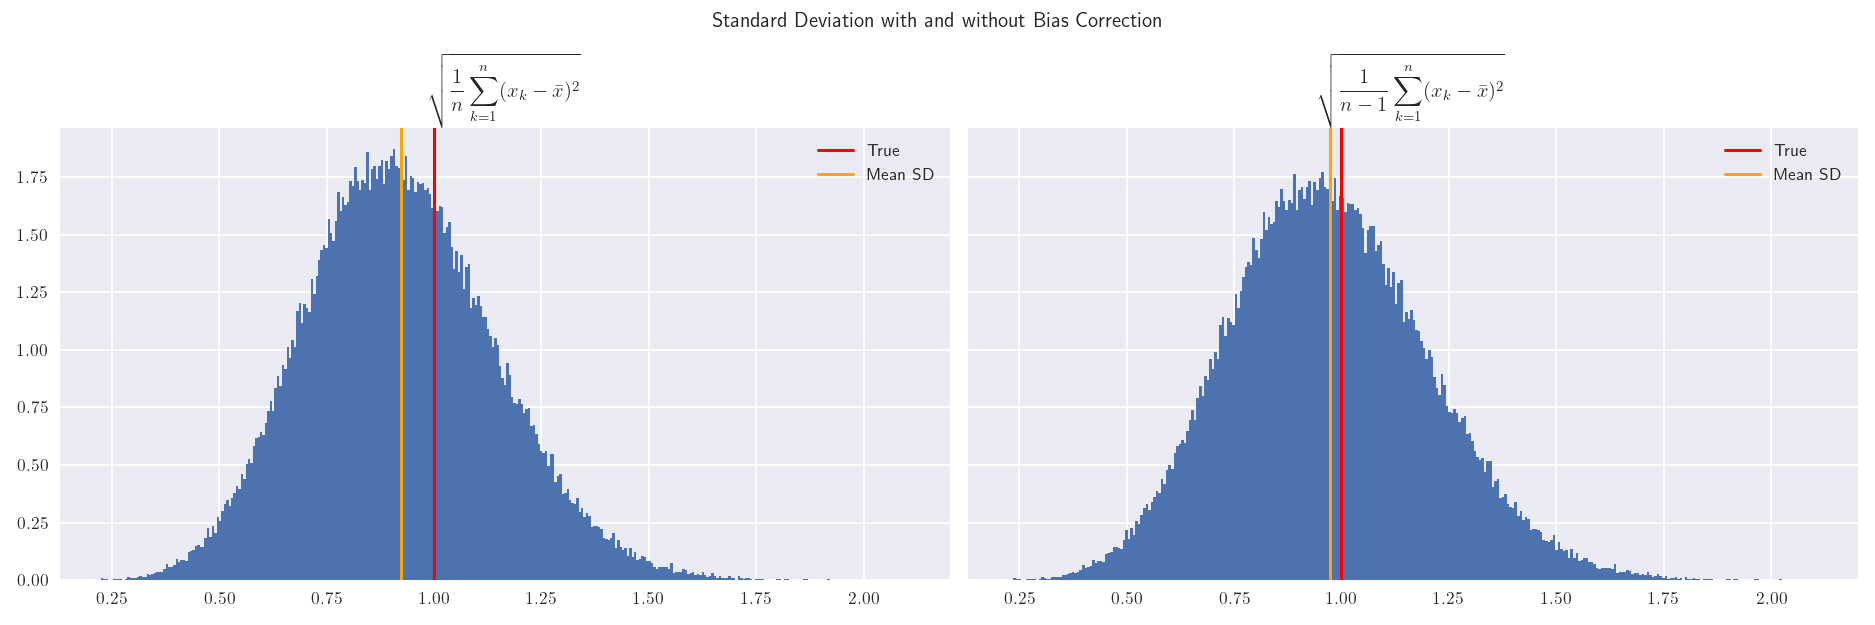
\includegraphics[scale = 0.3]{\pathtoimages/ex3-8.png}
\end{figure}
\end{frame}

\begin{frame}
\frametitle{Sample Variance on YouTube}
\small 
There's a StatQuest about sample variance ({\small \url{https://www.youtube.com/watch?v=sHRBg6BhKjI}})!
\begin{center}
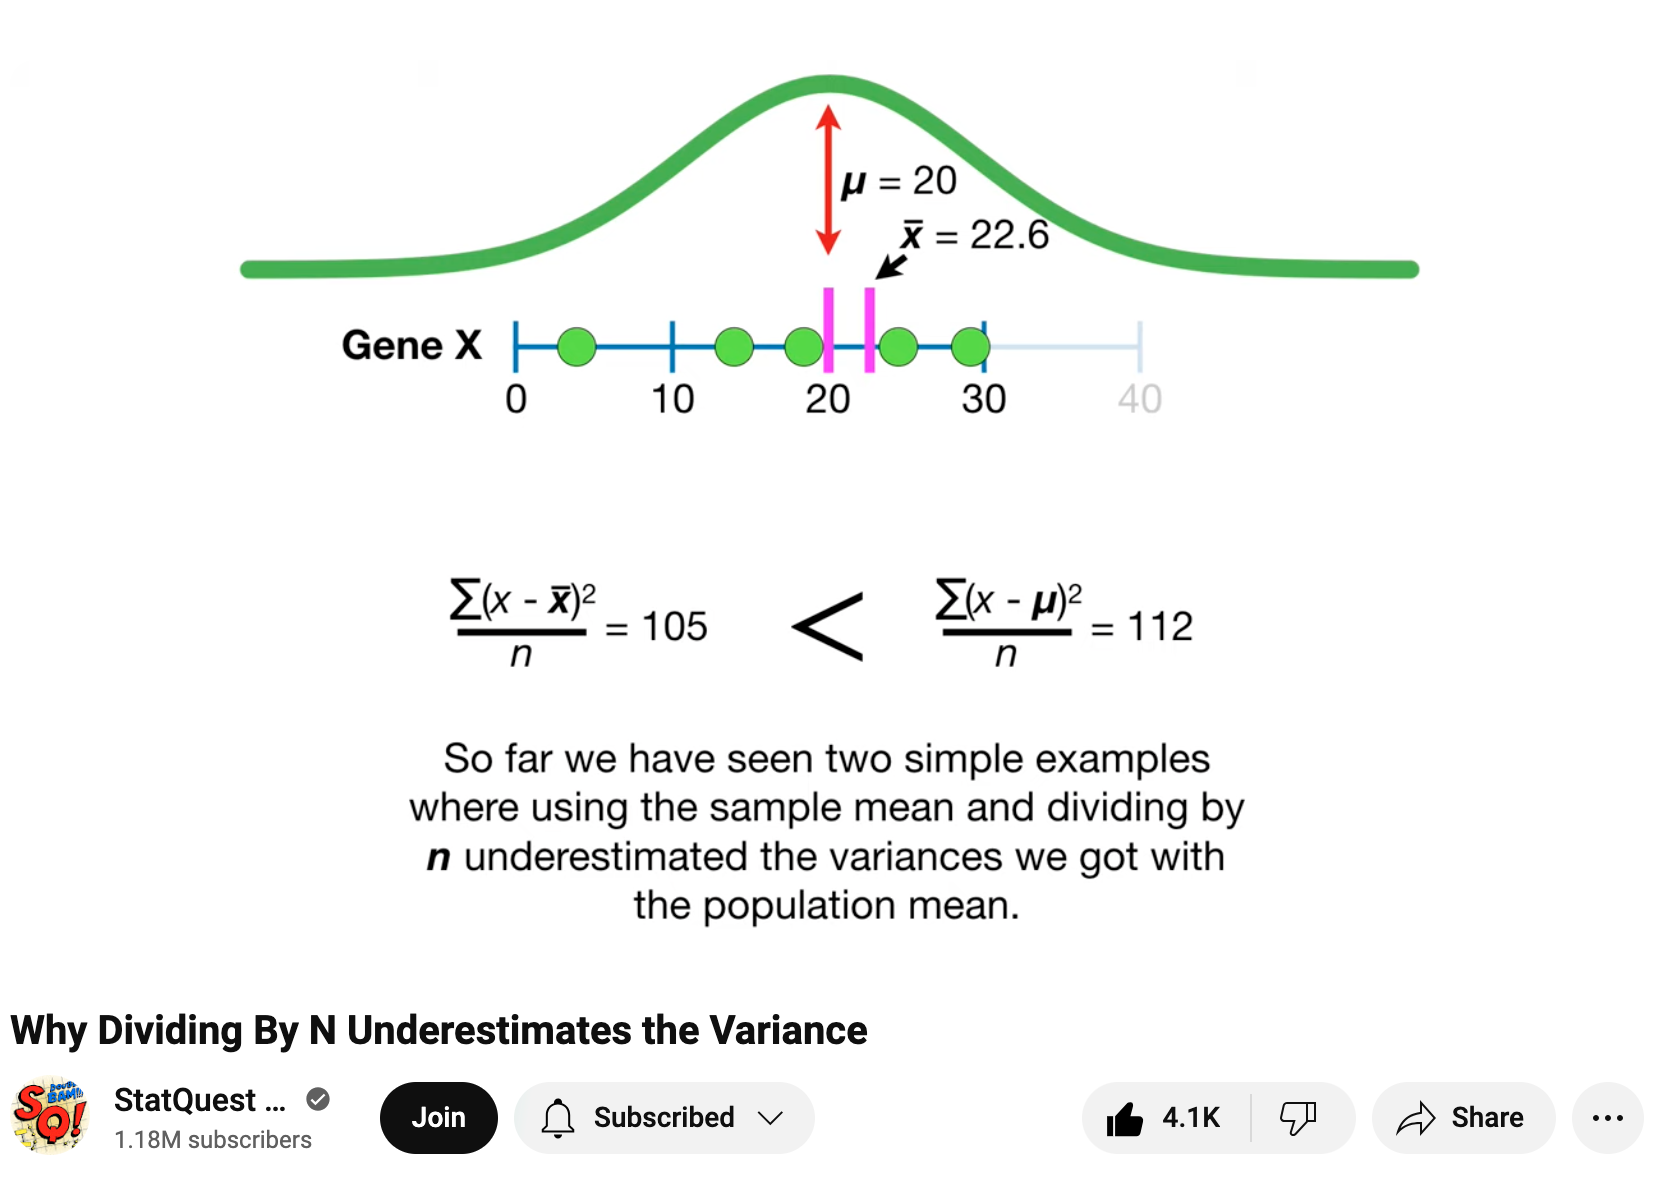
\includegraphics[scale = 0.25]{\pathtoimages/statquest-sample.png}
\end{center}

\end{frame}

\begin{frame}
\frametitle{Student's $t$-Distribution}
\begin{Definition}
Let $x_1, x_2,\ldots x_n\sim{\mathcal{N}(\mu, \sigma^2)}$ be independent and identically distributed samples. Then
$$
T = \frac{\bar{x} - \mu}{s/\sqrt{n}}
$$
follows a $t$-distribution with $n-1$ degrees of freedom. We often write $T \sim{t_{n-1}}$.
\end{Definition}
For $n > 30$ the $t$-distribution is approximately equal to a normal distribution. As a result, this distribution is only relevant for small samples. 
\end{frame}

\begin{frame}[t]
\frametitle{Hypothesis Testing with Unknown Variance}
\tiny
\begin{Example}
You sample the numbers 8, 0.5, 0, and $-0.5$ from a normal distribution. Perform a hypothesis test to determine whether the mean of the distribution is larger than 0 at a significance level of 10\%. Note: If $T\sim{t_3}$, then $P(T > 1.638) \approx 10\%$.
\end{Example}

\end{frame}

\begin{frame}[t]
\frametitle{Hypothesis Testing Proportions}
\tiny
\begin{Example}
You flip a coin 100 times and it lands heads 65 times. Perform a hypothesis test to determine whether the probability of landing heads is statistically different from 50\% at a 95\% confidence level.
\end{Example}


\end{frame}

\begin{frame}
\frametitle{Confidence Interval}
The population parameter lies in this interval with probability $1 - \alpha$.
\begin{itemize}
\item Known Variance: 
$$
\left(\bar{x} - z_{\alpha/2} \frac{\sigma}{\sqrt{n}}, \bar{x} + z_{1 - \alpha/2} \frac{\sigma}{\sqrt{n}}\right).
$$
\item Unknown Variance: 
$$
\left(\bar{x} - t_{\alpha/2} \frac{s}{\sqrt{n}}, \bar{x} + t_{1 - \alpha/2} \frac{s}{\sqrt{n}}\right).
$$ 
Degrees of freedom are $n-1$.
\item Proportion: 
$$
\left(\hat{p} - z_{\alpha/2}\sqrt{\frac{\hat{p}(1 - \hat{p})}{n}}, \hat{p} + z_{1 - \alpha/2} \sqrt{\frac{\hat{p}(1 - \hat{p})}{n}}\right).
$$
\end{itemize}
\end{frame}



\end{document}
